% documentclass options:
% ngerman is needed for hyphenation if the thesis contains parts written in German
% BCOR is binding correction
% if you'd rather have a one sided thesis, add `oneside' to the documentclass
\documentclass[11pt,
  a4paper,
  % parskip=half, % This is some extra vertical space between paragraphs, the suggestion is 2cm which is really ugly, so we use what koma script gives us
  % you can also set it to full for even more space. But there is a bad tex style decision: parskip also changes the spacing between listitems such as
  % enumerate and itemize. For this purpose we include the enumitem package and set itemsep=.5em, of course you can change this
  BCOR=10mm,
  english]{book}
\usepackage[english]{babel} % If you write mainly in english change order to ngerman, english
% Include of titling must happen before \title etc.
% that's why it's not in setup.tex
\usepackage{titling}

\title{Distributed Assertion Checking in Smart Contracts --- Preparation and Development of a Toolchain for the Tezos Blockchain}
\author{Tamara Bernhardt}

% include all packages and define commands in setup.tex

%------------------------------------------------------------------------------
%       package includes
%------------------------------------------------------------------------------
    % font encoding is set up for pdflatex, for other environments see
    % http://tex.stackexchange.com/questions/44694/fontenc-vs-inputenc
    \usepackage[T1]{fontenc}  % 8-bit fonts, improves handling of hyphenations
    \usepackage{lmodern}
    \usepackage[utf8x]{inputenc}
    % provides `old' commands for table of contents. Eases the ability to switch
    % between book and scrbook
    % cross-referencing
    \usepackage{xr}


    % ------------------- layout, default -------------------
    % adjust the style of float's captions, separated from text to improve readabilty
    \usepackage[labelfont=bf, labelsep=colon, format=hang, textfont=singlespacing]{caption}
    % With format = hang your caption will look like this:
    % Figure 1: Lorem ipsum dolor sit amet,
    %           consectetuer adipiscing elit.
    %           Ut purus elit, vestibulum
    % If you instead want
    % Figure 1: Lorem ipsum dolor sit amet,
    % consectetuer adipiscing elit. Ut purus
    % elit, vestibulum
    % change to format=plain
    \usepackage{chngcntr}  % continuous numbering of figures/tables over chapters
    \counterwithout{equation}{chapter}
    \counterwithout{figure}{chapter}
    \counterwithout{table}{chapter}

    % Uncomment the following line if you switch from scrbook to book
    % and comment the setkomafont line
    \usepackage{titlesec}  % remove "Chapter" from the chapter title
    \titleformat{\chapter}[hang]{\bfseries\huge}{\thechapter}{2pc}{\huge}
    % \setkomafont{chapter}{\normalfont\bfseries\huge}

    \usepackage{setspace}  % Line spacing
    \onehalfspacing
    % \doublespacing  % uncomment for double spacing, e.g. for annotations in correction

    % ------------------- functional, default-------------------
    \usepackage{natbib}
    \usepackage[dvipsnames]{xcolor}  % more colors
    \usepackage{array}  % custom format per column in table - needed on the title page
    \usepackage{graphicx}  % include graphics
    \usepackage{subfig}  % divide figure, e.g. 1(a), 1(b)...
    \usepackage{amsmath}  % |
    \usepackage{amsthm}   % | math, bmatrix etc
    \usepackage{amsfonts} % |
    \usepackage{calc}  % calculate within LaTeX
    \usepackage[unicode=true,bookmarks=true,bookmarksnumbered=true,
                bookmarksopen=true,bookmarksopenlevel=1,breaklinks=false,
                pdfborder={0 0 0},backref=false,colorlinks=false]{hyperref}
	\usepackage{listings}
	\usepackage{tabularx}
	\usepackage{makecell}
	\usepackage{upquote}

    %==========================================
    % You might not need the following packages, I only included them as they
    % are needed for the example floats
    % ------------------- functional, custom -------------------
    \usepackage{algorithm,algpseudocode}
    \usepackage{bm}  % bold greek variables (boldmath)
    \usepackage{tikz}
    \usetikzlibrary{positioning}  % use: above left of, etc

    % Improves general appearance of the text
    \usepackage[protrusion=true,expansion=true, kerning]{microtype}
    \usepackage{enumitem}

	\usepackage{csquotes}
	\usepackage{scrhack}

%------------------------------------------------------------------------------
%       (re)new commands / settings
%------------------------------------------------------------------------------
    % ----------------- referencing ----------------
    \newcommand{\secref}[1]{Section~\ref{#1}}
    \newcommand{\chapref}[1]{Chapter~\ref{#1}}
    \renewcommand{\eqref}[1]{Equation~(\ref{#1})}
    \newcommand{\figref}[1]{Figure~\ref{#1}}
    \newcommand{\tabref}[1]{Table~\ref{#1}}
    \newcommand{\lstref}[1]{Listing~\ref{#1}}
    %\newcommand{\algref}[1]{Algorithm~\ref{#1}}
    \newcommand*{\captionsource}[2]{%
  		\caption[{#1}]{%
    	#1%
    	\\\hspace{\linewidth}%
    	Source: #2%
  		}%
	}

    % ------------------- colors -------------------
    \definecolor{darkgreen}{rgb}{0.0, 0.5, 0.0}
    % Colors of the Albert Ludwigs University as in
    % https://www.zuv.uni-freiburg.de/service/cd/cd-manual/farbwelt
    \definecolor{UniBlue}{RGB}{0, 74, 153}
    \definecolor{UniRed}{RGB}{193, 0, 42}
    \definecolor{UniGrey}{RGB}{154, 155, 156}
    \definecolor{cverbbg}{gray}{0.93}

    % ------------------- layout -------------------
    % prevents floating objects from being placed ahead of their section
    \let\mySection\section\renewcommand{\section}{\suppressfloats[t]\mySection}
    \let\mySubSection\subsection\renewcommand{\subsection}{\suppressfloats[t]\mySubSection}


    % ------------------- marker commands -------------------
    % ToDo command
    \newcommand{\todo}[1]{\textbf{\textcolor{red}{(TODO: #1)}}}
    \newcommand{\extend}[1]{\textbf{\textcolor{darkgreen}{(EXTEND: #1)}}}
    % Lighter color to note down quick drafts
    \newcommand{\draft}[1]{\textbf{\textcolor{NavyBlue}{(DRAFT: #1)}}}
    \newcommand{\move}[1]{\textbf{\textcolor{Orange}{(MOVE?: #1)}}}


    % ------------------- math formatting commands -------------------
    % define vectors to be bold instead of using an arrow
    \renewcommand{\vec}[1]{\mathbf{#1}}
    \newcommand{\mat}[1]{\mathbf{#1}}
    % tag equation with name
    \newcommand{\eqname}[1]{\tag*{#1}}


    % ------------------- pdf settings -------------------
    % ADAPT THIS
    \hypersetup{pdftitle={\thetitle},
                pdfauthor={\theauthor},
                pdfsubject={Master's thesis at the Albert Ludwig University of Freiburg},
                pdfkeywords={blockchain, smart contract},
                pdfpagelayout=OneColumn, pdfnewwindow=true, pdfstartview=XYZ, plainpages=false}


    %==========================================
    % You might not need the following commands, I only included them as they
    % are needed for the example floats

    % ------------------- Tikz styles -------------------
    \tikzset{>=latex}  % arrow style


    % ------------------- algorithm ---------------------
    % Command to align comments in algorithm
    \newcommand{\alignedComment}[1]{\Comment{\parbox[t]{.35\linewidth}{#1}}}
    % define a foreach command in algorithms
    \algnewcommand\algorithmicforeach{\textbf{foreach}}
    \algdef{S}[FOR]{ForEach}[1]{\algorithmicforeach\ #1\ \algorithmicdo}

    % line spacing should be 1.5
    \renewcommand{\baselinestretch}{1.5}

    % set distance between items in a list, for more details see the
    % enumitem package: https://www.ctan.org/pkg/enumitem
    \setlist{itemsep=.5em}

% Copyright 2017 Sergei Tikhomirov, MIT License
% https://github.com/s-tikhomirov/solidity-latex-highlighting/

\usepackage{listings, xcolor}

\definecolor{verylightgray}{rgb}{.97,.97,.97}

\lstdefinelanguage{Solidity}{
	keywords=[1]{anonymous, assembly, assert, balance, break, call, callcode, case, catch, class, constant, continue, constructor, contract, debugger, default, delegatecall, delete, do, else, emit, event, experimental, export, external, false, finally, for, function, gas, if, implements, import, in, indexed, instanceof, interface, internal, is, length, library, log0, log1, log2, log3, log4, memory, modifier, new, payable, pragma, private, protected, public, pure, push, require, return, returns, revert, selfdestruct, send, solidity, storage, struct, suicide, super, switch, then, this, throw, transfer, true, try, typeof, using, value, view, while, with, addmod, ecrecover, keccak256, mulmod, ripemd160, sha256, sha3}, % generic keywords including crypto operations
	keywordstyle=[1]\color{blue}\bfseries,
	keywords=[2]{address, bool, byte, bytes, bytes1, bytes2, bytes3, bytes4, bytes5, bytes6, bytes7, bytes8, bytes9, bytes10, bytes11, bytes12, bytes13, bytes14, bytes15, bytes16, bytes17, bytes18, bytes19, bytes20, bytes21, bytes22, bytes23, bytes24, bytes25, bytes26, bytes27, bytes28, bytes29, bytes30, bytes31, bytes32, enum, int, int8, int16, int24, int32, int40, int48, int56, int64, int72, int80, int88, int96, int104, int112, int120, int128, int136, int144, int152, int160, int168, int176, int184, int192, int200, int208, int216, int224, int232, int240, int248, int256, mapping, string, uint, uint8, uint16, uint24, uint32, uint40, uint48, uint56, uint64, uint72, uint80, uint88, uint96, uint104, uint112, uint120, uint128, uint136, uint144, uint152, uint160, uint168, uint176, uint184, uint192, uint200, uint208, uint216, uint224, uint232, uint240, uint248, uint256, var, void, ether, finney, szabo, wei, days, hours, minutes, seconds, weeks, years},	% types; money and time units
	keywordstyle=[2]\color{teal}\bfseries,
	keywords=[3]{block, blockhash, coinbase, difficulty, gaslimit, number, timestamp, msg, data, gas, sender, sig, value, now, tx, gasprice, origin},	% environment variables
	keywordstyle=[3]\color{violet}\bfseries,
	identifierstyle=\color{black},
	sensitive=false,
	comment=[l]{//},
	morecomment=[s]{/*}{*/},
	commentstyle=\color{gray}\ttfamily,
	stringstyle=\color{red}\ttfamily,
	morestring=[b]',
	morestring=[b]"
}

\lstdefinestyle{Solidity}{
	backgroundcolor=\color{verylightgray},
	extendedchars=true,
	basicstyle=\footnotesize\ttfamily,
	showstringspaces=false,
	showspaces=false,
	numbers=left,
	numberstyle=\footnotesize,
	numbersep=9pt,
	tabsize=2,
	breaklines=true,
	showtabs=false,
	captionpos=b
}

\usepackage{listings, xcolor}

\definecolor{verylightgray}{rgb}{.97,.97,.97}

\lstdefinelanguage{Michelson}{
	keywords=[1]{parameter, storage, code},
	keywordstyle=[1]\color{blue}\bfseries,
	keywords=[2]{address, unit, never, bool, int, nat, string, chain_id, bytes, mutez, key_hash, key, signature, timestamp,
	option, or, pair, list, set, operation, ticket, lambda, map, big_map, sapling_transaction, sapling_state, bls12_381_g1,
	bls12_381_g2, bls12_381_fr},	% types; money and time units
	keywordstyle=[2]\color{teal}\bfseries,
	keywords=[3]{Do, call, assert},
	keywordstyle=[3]\color{violet}\bfseries,
	identifierstyle=\color{black},
	sensitive=false,
	comment=[l]{//},
	morecomment=[s]{(*}{*)},
	commentstyle=\color{gray}\ttfamily,
	stringstyle=\color{red}\ttfamily,
	morestring=[b]',
	morestring=[b]"
}

\lstset{
	language=Michelson,
	backgroundcolor=\color{verylightgray},
	extendedchars=true,
	basicstyle=\footnotesize\ttfamily,
	showstringspaces=false,
	showspaces=false,
	numbers=left,
	numberstyle=\footnotesize,
	numbersep=9pt,
	tabsize=2,
	breaklines=true,
	showtabs=false,
	captionpos=b
}

\usepackage{listings, xcolor}

\definecolor{verylightgray}{rgb}{.97,.97,.97}

\lstdefinelanguage{Assertion}{
	keywords=[1]{entrypoint, assert, if, else, true, false, forall, exists},
	keywordstyle=[1]\color{blue}\bfseries,
	keywords=[2]{address, unit, never, bool, int, nat, string, chain_id, bytes, mutez, key_hash, key, signature, timestamp,
	option, or, pair, list, set, operation, lambda, map, big_map},	% types; money and time units
	keywordstyle=[2]\color{teal}\bfseries,
	keywords=[3]{left, right, some, none, cons, nil, _},
	keywordstyle=[3]\color{violet}\bfseries,
	identifierstyle=\color{black},
	sensitive=false,
	comment=[l]{//},
	morecomment=[s]{(*}{*)},
	commentstyle=\color{gray}\ttfamily,
	stringstyle=\color{red}\ttfamily,
	morestring=[b]',
	morestring=[b]"
}


\begin{document}
    \pagestyle{empty} % no header and no page number
    % disable hyper links to remove warning "destination with same identifier"
    % this means within this section nothing can be referenced with a hyperlink
    \hypersetup{pageanchor=false}

    % enable/disable, depending on your chosen language
    
\begin{titlepage}
\begin{center}

\newcommand{\HorizontalLine}{\rule{\linewidth}{0.3mm}}

{\Large Master's Thesis}\\[1.3cm]


% _____________________________________________________________________________
\HorizontalLine \\[0.4cm]
% Write your title in a fancy way like this if you want to customize it, otherwise simply let tex do it for you
% \begin{spacing}{3}
%     {\huge \bfseries The Long, Long } \\
%     {\huge \bfseries Long Long} \\
%     {\huge \bfseries Title}\\
% \end{spacing}
{ \huge \bfseries \thetitle }
\HorizontalLine \\[1.5cm]
% _____________________________________________________________________________


{\Huge \theauthor} \\[2cm]


\begin{tabular}[hc]{>{\huge}l >{\huge}l}
  Examiner: & Prof. Dr. Peter Thiemann \\[0.3cm]
  2nd Examiner: & Prof. Dr. Andreas Podelski \\[0.3cm]
  Advisers: & \todo{lla} \\[1.2cm]
\end{tabular}
\vfill  % move the following text to the bottom

\Large {
    Albert-Ludwigs-University Freiburg\\
    Faculty of Engineering\\
    Department of Computer Science\\
    Chair for Programming Languages\\[1cm]
}
\end{center}
\end{titlepage}

\thispagestyle{empty}
% title page back
\ \vfill \ \\  % at least one space required before vfill
\
\textbf{Writing period}            \smallskip{} \\
01.\,10.\,2020 -- 31.\,03.\,2021 \todo   \bigskip{} \\
\
\textbf{Examiner}                  \smallskip{} \\
Prof. Dr. Peter Thiemann               \bigskip{} \\
\
\textbf{2nd Examiner}                  \smallskip{} \\
Prof. Dr. Andreas Podelski


    \pagestyle{plain} % remove chapter name from top, page number at the bottom
    % use \pagestyle{headings} for having the chapter on top of the pages
    % if you wang a more fancy header use \usepackage[automark,headsepline]{scrlayer-scrpage}
    % and read about it in the KOMA script documentation, https://www.ctan.org/pkg/koma-script
    \frontmatter  % roman page numbers
    % official declaration from the examination office; to be sure double
% check the wording on their website
% (https://www.tf.uni-freiburg.de/studies/exams/thesis/thesis_formatting.html#erklaerung)

\chapter*{Declaration}

I hereby declare that I am the sole author and composer of my thesis and that no other sources or learning aids, other than those listed, have been used. Furthermore, I declare that I have acknowledged the work of others by providing detailed references of said work.  \newline
I hereby also declare that my Thesis has not been prepared for another examination
or assignment, either wholly or excerpts thereof.
\\[3\normalbaselineskip]
\begin{tabular}{p{\textwidth/2} l}
  \rule{\textwidth/3}{0.4pt}   &   \rule{\textwidth/3}{0.4pt} \\
  Place, Date                  &   Signature
\end{tabular}

    \chapter*{Abstract}
Modern blockchains provide a platform for building sophisticated applications with smart contracts. Because transactions are processed at every node in the network, the quantity and complexity of computations, which can be performed by smart contracts, are limited. Furthermore, complex contracts can generate high transaction costs for the user. To overcome this limitation and improve cost efficiency, blockchain-based applications could move computations to an off-chain component and only process the result on the blockchain. This thesis proposes a processing model for the Tezos blockchain, which engages the validators of the network in a distributed effort to verify a submitted off-chain computation. Based on a specification of properties, the validators are challenged to find a counterexample by asserting these properties for independent subsets of the result. This reduces the computational effort on the blockchain to the verification of the result, rather than the computation of the result itself. Moreover, by implementing a distributed scheme, each node only processes a fraction of the verification. For this processing model, this thesis contributes a domain-specific language to express explicit assertions for off-chain computations and specifies a processing pipeline to transform and compile these assertions into smart contracts. These contracts conduct a point-wise search for a counterexample and are called during the verification mechanism. The provided proof-of-concept implementation of this pipeline targets Tezos, but is by design extendible for other blockchains supporting smart contracts.
    \tableofcontents
    \listoffigures
    \lstlistoflistings
    \hypersetup{pageanchor=true}  % re-enable hyperlinking

    \mainmatter  % Arabic page numbers
    \chapter{Introduction}\label{chap:introduction}
Headed by Bitcoin in 2009 \cite{bitcoin-whitepaper}, the first generation of blockchain technology emerged in form of cryptocurrencies. However, their transactions are mostly limited to simple monetary transactions or registration of assets or ownerships \cite{alharby_blockchain_2017}. More recent blockchains, considered as the second generation, aim to provide a platform for building more sophisticated and complex applications on top of the technology. Some prominent examples for such blockchains are Ethereum \cite{eth-whitepaper}, Tezos \cite{goodman_tezos_2014} or Cardano \cite{cardano_essay}, which plans to introduce smart contracts in an update this year \cite{cardano_alonzo}. Blockchain-based applications are built with smart contracts, programs written in Turing-complete languages. Running a smart contract, though, generates costs proportional to the amount and complexity of computations, as well as its storage usage \cite{alharby_blockchain_2017}. These fees, often measured in a unit called ``gas'', have to be paid for by the user in order to compensate the miners for their efforts \cite{narayanan_bitcoin}. This creates a powerful incentive to keep smart contracts simple and efficient, while in reality, meaningful applications still might need to perform some resource intensive computations. Not only can such applications generate unsustainable costs when executed on the blockchain, but may also reach gas limits imposed by the blockchain's protocol. \\
In order to avoid these costs and restrictions, such an application could perform some computations outside of the blockchain context (i.e., off-chain) and only submit the results to a smart contract as an input parameter for further processing or recording. By trusting that the submitted results are correct, this approach raises both safety and security issues. Invalid results can be submitted unintentionally as a result of a wrong computation, or a third party may pass them intentionally to cause harm or take advantage. Consequently, submitted parameters should be checked for assumed properties before the smart contract is executed. Although in many cases, verifying a solution takes less time than computing the result itself (cf. NP-hard problems \cite{nph_problems} or sorting algorithms \cite{review_sorting}\cite{cpp_issorted}), the generated costs for checking the validity increase with the size of the input. \\
Consider the smart contract \texttt{Example}, which is shown in \lstref{lst:prime} and features a function \texttt{f}. The function takes an input value \texttt{p} of type integer and should make use of the assumption that \texttt{p} is a prime number.
\begin{lstlisting}[caption=Smart contract with a function that expects a prime number \cite{thiemann_2020}, numbers=none, language=Solidity, label=lst:prime]
contract Example {
	function f ( int p ) public {
	// assume p is prime
	...
	}
}
\end{lstlisting}
This assumption ``$p$ is a prime number'' can be expressed with the following explicit assertion in predicate logic: 
\begin{equation}\label{eq:prime}
    (\forall n) (2 \le n \le \sqrt{p}) \Rightarrow (p \% n) \neq 0
\end{equation}
To check whether this property holds for $p$, the contract has to execute a loop over the range $[2, \sqrt{p}]$. Assuming that computing the body of the loop takes constant time, this test has a time complexity of $\mathcal{O}(\sqrt{p})$ and therefore generates costs linear in $\sqrt{p}$ on top of the cost for executing the actual contract. Thus, a mechanism is required that allows the smart contract to make use of the result computed by an off-chain source, without having to check its validity locally with scaling costs.

\section{A distributed approach for assertion checking}
A more efficient way to solve the issue at hand could be to engage the validators of the blockchain into a distributed effort to find a counterexample. If no counterexample could be found by any validator, the assumption is considered to be valid and the execution of the contract may resume. On the other hand, an identified counterexample is made public on the peer-to-peer network and thus cancels the contract execution (i.e., the transaction fails). \\
In order to find a counterexample, the formula in \eqref{eq:prime} has to be transformed to its negation:
\begin{equation}\label{eq:prime_neg}
	(\exists n) (2 \le n \le \sqrt{p}) \wedge (p \% n) = 0
\end{equation}

Each validator then checks the inverse property $(p \% n) = 0$ point-wise for some random $n$ within the given boundaries $2 \le n \le \sqrt{p}$. If a validator finds a counterexample, i.e., a value for $n$ where the reminder is $0$, it posts an objection to the network. For each involved validator, the constant cost of generating one random number and calculating one division have to be paid, which is independent from $p$. \\
However, distributed assertion checking is not only applicable for parameters or properties of dynamic size. Function \texttt{find} of contract \texttt{Sorted}, shown in \lstref{lst:sorted}, expects a statically sized array of integers and a single integer value. In order to find the value \texttt{v} in \texttt{a} more efficiently, the array is assumed to be sorted. 

\begin{lstlisting}[caption=Smart contract expecting a sorted array \cite{thiemann_2020}, numbers=none, language=Solidity, label=lst:sorted]
contract Sorted {
  function find ( int [50] a , int v ) public {
    // assume a is sorted
    ...
  }
}
\end{lstlisting}

The explicit assertion of this assumption (in the variant of an ascending sorting) can be expressed as follows in predicate logic:
\begin{equation}\label{eq:sorted}
	(\forall n) (0 \leq n < |a| - 1) \Rightarrow a[n] \leq a[n+1]
\end{equation}

Even though the assertion can be checked in a loop in $\mathcal{O}(1)$, the constant factor is not negligible. Hence, the same approach can be applied here by considering the negation and have the validators search for counterexamples, checking random values for $n$:
 
\begin{equation}\label{eq:sorted_neg}
	(\exists n) (0 \leq n < |a| - 1) \wedge a[n] > a[n+1]
\end{equation}

Since the validators sample the domain randomly, the absence of a counterexample doesn't prove that the assumption is correct; the validation is only probabilistic and the reliability depends on the number of validators in the network. This corresponds to the principle of Bloom filters, where a queried element is either ``certainly not'' or ``possibly'' a member of a defined set \cite{blustein_bloom_2002}. In the case of assertion checking, we consider the assumption to be either definitely not or possibly valid. The probability of false positives in Bloom filters is an approximate function of the filter size and the number of inserted elements, supposing an optimal number of hash functions have been implemented. Tuning these parameters is a trade-off between making the filter more reliable, i.e., lowering its error rate, and space efficiency \cite{blustein_bloom_2002}. The same applies, with some reservations, to distributed assertion checking: less samples keep the gas consumption to a minimum, whereas more samples increase the probability that an existing counterexample is found. Referring to the example of sorted lists,  the probability of false positives depends on the size of the list $a$ and the number of validators $m$.

The importance of the former parameter becomes apparent when considering the worst case scenario of the same example. Assuming the array is unsorted at exactly one position - the probability that the each of the $m$ validators independently check this position is $\frac{1}{|a|}$, whereas the probability of all of them checking any other position $\frac{|a|-1}{|a|}$. If the random generator chooses each value for $n$ independently from a uniform distribution, the probability that the counterexample is not detected by any validator converges to 0 if the number of validators approaches infinity \cite{thiemann_2020}:
\begin{equation}\label{eq:limes_validators}
	\lim_{m\to\infty} \left(\frac{|a|-1}{|a|}\right)^m = 0
\end{equation}

\section{Objective}
This thesis proposes a model for the portrayed approach of a distributed assertion checking scheme, to make more efficient use of off-chain computations. In this model, results of such computations are validated on-chain by the validators of the network. In order to do so, they invoke assertion smart contracts which point-wise check whether the result satisfies certain properties. When claiming an assertion failure, a validator publishes a counterexample to be scrutinized by the other validators. If they come to a consensus about the invalidity, the result is rejected. Provided that the assertion is cheaper than the computation itself, the purpose of this proposal is not only to reduce financial costs for the users, but also to overcome limitations in scalability. 

The realisation of such assertions consists of an off-chain and an on-chain component. The off-chain component is a toolchain to specify, integrate and generate assertion contracts that can be deployed to the blockchain. It defines of a domain-specific language which allows developers to specify assertions for each entrypoint of a Smart Contract. The toolchain implements a pipeline which transforms the assertion, links it with the Smart Contract and translates it to the Smart Contract language. \\
The on-chain component consists of an amendment of the blockchain protocol to include transactions that can trigger the distributed execution of assertions and implement a consensus mechanism for counterexamples. 

The focus of this thesis is put primarily on the off-chain component, but it elaborates on the protocol design where necessary.  Even though efforts were made to keep the design as generic and re-usable as possible, the implementation targets the Tezos blockchain and its built-in contract language Michelson. On the basis of the design and implementation for Tezos, the thesis evaluates the efficiency and incurred costs of this approach and discusses whether, and under which conditions, they can be competitive versus a centralized assertion approach.

\section{Related work}


\section{Structure overview}
The structure of this thesis is as follows: in the first instance, \chapref{chap:use_cases} defines a set of logical formulas suitable for distributed assertion checking. Given this set, it demonstrates various practical use-cases for such properties and formalizes the costs of checking them locally, s.t. they can later be referenced to assess the efficiency of the distributed approach. \chapref{chap:offline} describes the generic aspects of the off-chain design and infrastructure, i.a. the definition of a syntax to express assertions on top of the logical formulas and how they are transformed to code that checks for counterexamples. Additionally, it analyses the effectiveness of the statistical validation for a given input and provides a formula to compute the lower bound of validators necessary to obtain a reliable result. Subsequently, \chapref{chap:offline_tezos} gives a brief introduction to Tezos, before it covers target specific aspects of the off-chain design. Besides identifying necessary extensions to Michelson's instruction set and virtual machine, it explores various orchestration strategies between assertion and contract code. The chapter closes with a cost analysis of distributed assertion checking on Tezos with the chosen orchestration strategy. In conclusion, the last chapter recaps the achieved results, 
addresses open questions or issues and provides an outlook on upcoming work on this topic.
    \chapter{Use-case analysis}\label{chap:use_cases}
The introduction argued, that validating properties on input parameters can become costly when data structures (such as arrays), certain data types (such as byte sequences) or a range of values have to be iterated. It showed examples for such properties and identified logical formulas containing universal quantification as amenable for distributed assertion checking. Through its domain of discourse, the quantification spans an iteration space whose elements can be checked independently by the validators. As a matter of fact, the same is also valid for existential quantification, even though its negation has a different notion than that of its universal counterpart. The difference between the two is addressed later in this chapter.

The following section formally defines a set of applicable logical formulas for the basic implementation of the distributed assertion checking scheme. Given this set, section \secref{sec:examples} gives some more in-depth examples of such formulas. As a benchmark for the distributed scheme, the last section formalizes the cost incurred by checking formulas on Tezos locally.

\section{Definition of a set of logical formulas}\label{sec:formulae}
The set of formulas, which can be expressed in well-formed assertions, is given in \figref{fig:formulas}. This corresponds, with some restrictions, to the language of second-order predicate logic. Besides universal and existential quantifiers (with exactly one bound variable), the definition contains logical connectives, relational symbols, constant values of a numerical, string or boolean type, variables and the functional symbols for basic arithmetic operations. This set of symbols is rather generic and should be valid for any target blockchain. Specific to the target blockchain are the sets of types $t$ and functional symbols $f$. These can only contain types and operations, which can be translated to instructions of the respective Smart Contract language and interpreted by the blockchain's virtual machine (VM). As an example, the primitive types in Michelson are \texttt{string}, \texttt{nat}, \texttt{int}, \texttt{bytes}, whereas Ethereum's Smart Contract language Solidity  \cite{solidity_docs} additionally supports an \texttt{enum} type and fixed-point numbers.
\begin{align*}
    t &::= \text{primitive data types (existing in the blockchain VM)} \\
    \sigma &::= \forall \mid \exists \\
    \Theta &::= \Phi \mid \sigma (x:t) \Theta \\
    \Phi,\Psi &::= \neg\Phi \mid \Phi \Rightarrow \Psi \mid \Phi\wedge\Psi \mid
    				\Phi\vee\Psi \mid \Phi \oplus \Psi \mid M \rho N \\
    \rho &::= < \mid > \mid \le \mid \ge \mid = \mid \ne \\
    M, N &::= x \mid c \mid M \odot N  \mid f (\overline M) \\
    \odot &::= +\mid -\mid * \mid / \mid \% \\
    c &::= \text{numerical value} \mid string \mid \top \mid \bot \\
    f &::= \text{operations (existing in the blockchain VM)}
\end{align*}
\begingroup\vspace*{-\baselineskip}
\captionof{figure}{Set of logical formulas amenable to distributed assertion checking (based on \cite{thiemann_2020})}
\label{fig:formulas}
\vspace*{\baselineskip}\endgroup

\section{Examples and special cases}\label{sec:examples}
This section contains a subset of use-cases that were collected in collaboration with Julian Veigl for an intermediate report \cite{bernhardt_veigel_2020}. The selection of examples covers different types and compositions of quantifiers, demonstrates different meanings of their negations, identifies special cases and discusses their implications for the implementation of distributed assertion checking.

\subsection{Two numbers are coprime}\label{sec:coprime}
The greatest common divisor ($gcd$) of two non-zero integers $a$ and $b$ is the largest integer that divides both evenly \cite{hardy2008introduction}. A more specific $gcd$-problem is finding two numbers which are coprime, meaning their greatest common divisor is one, i.e., $gcd(a, b) = 1$. In order to verify that two numbers are coprime, it has to be verified that there is no $gcd > 1$, hence the property of coprimeness can be expressed with the following formula in predicate logic:
\begin{equation}\label{eq:coprime-universial}
    (\forall n : int) (2 \le n \le \min(a,b)) \Rightarrow \neg((a \mathbin{\%} n) = 0 \land (b \mathbin{\%} n) = 0)
\end{equation}
Assuming it takes constant time to calculate the two remainders, checking whether two numbers satisfy this property takes linear time, i.e. $\mathcal{O}(n)$, and depends on the size of the smaller number.

When checking the assumption through a distributed effort instead, the validators consider its negation:
\begin{equation}\label{eq:coprime-existential}
    (\exists n : int) (2 \le n \le \min(a,b)) \land (a \mathbin{\%} n) = 0 \land (b \mathbin{\%} n) = 0
\end{equation}
If, within the given domain, this condition is true for a random value for $n$, the respective validator has found a counterexample.

\subsection{Heap property}
Heaps \cite{dict_heap} are data structures based on trees and can appear in two varieties: min and max heaps. Both can be represented as binary trees and have to satisfy the heap property: in a max heap, any given node holds a value lower or equal than that of its parent, whereas in a min heap, it is greater or equal \cite{dict_heap_property}. Binary heaps are often implemented as an array, with the root of the tree stored at index 0. The relatives of a node \texttt{k} can be accessed as follows:
\begin{lstlisting}[language=Solidity, numbers=none, caption=Access a binary heap in array representation]
heap_array[(k-1)/2] // Get parent of node k
heap_array[(k*2)+1] // Get left child of node k
heap_array[(k*2)+2] // Get right child of node k
\end{lstlisting}
The min heap property for a binary heap stored in an array $a$, for instance, can be expressed in predicate logic with the following formula:
\begin{equation}\label{eq:heap-unversial}
  (\forall k : int) (1 \le k < |a|) \Rightarrow a[\lfloor(k-1)/2)\rfloor] \le a[k]
\end{equation}
The time complexity of checking whether $a$ satisfies the heap property depends on how the array is allocated. If it is dynamically sized, it takes $\mathcal{O}(n)$ in the size of the array, otherwise it takes constant time, i.e. $\mathcal{O}(1)$.  Similarly to the previous examples, counterexamples can be identified by considering the formula's negation:
\begin{equation}\label{eq:heap-unversial-neg}
  (\exists k : int) (1 \le k \le |a|) \land a[\lfloor(k-1)/2)\rfloor] > a[k]
\end{equation}

\subsection{Existential quantification - intersection of sets}\label{sec:existential}
So far, this thesis only considered formulas featuring universal quantification, for which the assertion scheme engaged the validators to find counterexamples. However, distributed assertion checking can not only be used to refute assumptions, but also to prove their validity. This is the case for formulas featuring existential quantification. As an example, consider the assumption that two sets $U$ and $V$ have a non-empty intersection, i.e., $U \cap V \neq \emptyset$. This assumption and its negation can be expressed in predicate logic by 
\begin{equation}\label{eq:intersect}
  (\exists i, \exists j) (0 \le i < |u|) \land (0 \le j < |v|) \Rightarrow u[i] = v[j]
\end{equation}
and
\begin{equation}\label{eq:intersect_neg}
  (\forall i, \forall j) (0 \le i < |u|) \land (0 \le j < |v|) \land u[i] \neq v[j]
\end{equation}
If the condition $u[i] \neq v[j]$ is false for random values of $i$ and $j$, it does not produce a counterexample --- it produces a proof for the validity of the assumption, because it identified an element that is present in both sets. In that case, the validator finding such a proof should publish an approval instead of a veto to the network. After an approval has been posted, and all validators have come to a consensus about the validity of the proof, the result is accepted. For the blockchain protocol, this implies that distributed refutation and validation have to be implemented as separate modi of assertion checking.

Concerning the complexity of this assertion, the property can be checked in $\mathcal{O}(|u|*|v|)$. By considering the cardinality of their union $n = |u|+|v|$, one can derive that the worst case occurs when both sets have the same size, i.e., $|u| = |v| = n/2$. This leads to a quadratic complexity $\mathcal{O}(n/2 * n/2) = \mathcal{O}(n^2/4) = \mathcal{O}(n^2)$.

\subsection{Nested quantification - SAT problems}
The previous example demonstrated that universal and existential quantification have to be handled differently. However, further special cases, caused by nested quantification, have to be considered as well. A nesting of the same type of quantifier, e.g. $\forall i \forall j$, can be considered as trivial. They are translated to code, which generates a random value for each predicate variable and checks for a counterexample or proof respectively. It becomes less trivial, if the nesting contains both universal and existential quantifiers. This section examines the cases of $\forall i \exists j$ and $\exists i \forall j$ on the basis of a contract that expects a solution for a boolean satisfiability problem (SAT).

Instances of SAT problems consist of a formula $F$ in propositional logic, and determine if there exists a variable assignment $\mathcal{A}$ to the values $true$ or $false$, s.t. the formula is satisfied ($\mathcal{A}(F) = 1$) \cite{Biere2009}. Modern SAT-solvers expect $F$ to be in conjunctive normal form (CNF), i.e., a conjunction of a set of clauses, where clauses are disjunctions of variables or their negations (called literals) \cite{cnf_math_encycl}. While finding an assignment $\mathcal{A}$ that satisfies $F$ is a NP-complete problem \cite{Biere2009}, verifying whether a given assignment satisfies the formula takes $\mathcal{O}(n*m)$, where $n$ is the number of clauses and $m$ the number of variables (in the worst case, every variable is present as a literal in each clause). In the case of k-SAT problems, where each clause contains at most k literals \cite{Biere2009}, the complexity is reduced to $\mathcal{O}(n)$.

\subsubsection{Encoding of variables, literals and clauses}
A SAT problem can be represented as a list of clauses $c$ and a variable assignment $\mathcal{A}$. To avoid having to handle the variables and their literals as strings, and thus optimize runtime and memory consumption, an encoding scheme \cite{sabablog} is used in the following.

Variables are encoded by a unique number starting from $0$ to $n-1$, where $n$ is the total number of variables. The positive and negative literals of a variable with id $x$ are encoded by the function
\begin{align*}
encode(x) =
\begin{cases}
  $2x$  & \text{if x is present as a positive literal}\\
  $2x+1$ & \text{if x is present as a negated literal}\\
\end{cases}   
\end{align*}
Consequently, checking whether a literal $y$ is positive or negative is a simple bit-wise $AND$ operation:
\begin{align*}
\texttt{isPositive(y) = y \& 1 == 0}
\end{align*}
Consider the following boolean formula and variable assignment:
\begin{align*}
F = (A \vee B) \wedge (B \vee \neg C) \text{, } \mathcal{A} = \{A \rightarrow false, B \rightarrow true, C \rightarrow false\}
\end{align*}
Following the encoding of variables given above, the list of variables $v=[A,B,C]$ occurring in $F$ is encoded as $v_{enc} = [0,1,2]$. If clauses are given as lists of literals, $F$ can be represented by the encoding $F_{enc} = [[0,2],[2,5]]$. Since the encoding of variables corresponds to their index in the list of variables, $\mathcal{A}$ can be passed as a list of booleans that maintains the same order of variables: $\mathcal{A}_{enc} = [False, True, False]$. If the blockchain's VM supports a respective data type, $\mathcal{A}$ can alternatively be represented with a more efficient bitarray. Lastly, the variable encoding $x$ of a literal $y$ is obtained by dividing its encoding by two, which corresponds to a bit-wise shift to the right:
\begin{align*}
\texttt{decode(y) = y >> 1}
\end{align*}

\subsubsection{Satisfiability in predicate logic - CNF}
Consider a contract that expects a SAT problem in CNF and a proposed assignment, both encoded as described above. Assuming that $F$ is a k-SAT instance, the assumption that $\mathcal{A}$ satisfies $F$ can be expressed in predicate logic as follows:
\begin{equation}\label{eq:cnf_sat}
\begin{aligned}
(\forall i : int, \exists j : int) &(0 \leq i < |F|) \wedge (0 \leq j < k) \\
&\Rightarrow ((isPositive(F[i][j]) \wedge \mathcal{A}[decode(F[i][j])]) \\
&\vee (\neg isPositive(F[i][j]) \wedge \neg \mathcal{A}[decode(F[i][j])])))
\end{aligned}
\end{equation}

In the previous examples, where formulas contained only a single quantifier, the predicate variables of the negated formula are replaced by a randomly generated number during assertion checking. Quantifiers thus are translated to random generators during the generation of target code. However, by checking a random literal in a random clause, the validator cannot make a definite statement about whether $\mathcal{A}$ satisfies $F$. Each clause has to be examined as a whole in order to verify, that the conjunction evaluates to true. Consequently, the distribution can only take place on the level of clauses, but not on the level of literals. Each validator thus has to check all literals of one random clause, which translates into a random generator for the outer quantifier, and a loop for the inner quantifier. Whether the assertion requires a proof or a counterexample can be derived from the outer quantifier, hence validators produce a counterexample in this case. \lstref{lst:cnf_test_code} shows the generated testing code of the CNF SAT problem, where \texttt{check} evaluates the negated condition. While formulas with a single quantifier simply translate to generating a random value and checking the condition, this code is more extensive. It requires a more sophisticated compiler, which can differentiate between different quantification compositions.

\begin{lstlisting}[label=lst:cnf_test_code, caption=Test code structure for single nested quantifiers, numbers=none]
i = random(0, size(F))
for (j : [0..k)):
  if not check( ... ):
    // property holds
    return true
// counterexample found
return false
\end{lstlisting}

Due to the loop, the cost incurred by one validator checking the assertion becomes, in the worst case, linear in the number of literals in the clause. An exception is the case of k-SAT instances, where the cost per validators remains constant, albeit with a factor $k$. 

\subsubsection{Satisfiability in predicate logic - DNF}\label{sec:dnf}
The same propositional formula, with the reversed quantification nesting $\exists i \forall j$, describes the assertion for the assumption $\mathcal{A}(F) = 1$, where $F$ is given in disjunctive normal form (DNF), i.e., a disjunction of conjunctions \cite{dnf_math_encycl}:
\begin{equation}\label{eq:dnf_sat}
\begin{aligned}
(\exists i : int, \forall j : int) \: &(0 \leq i < |F|) \wedge (0 \leq j < k) \\
&\Rightarrow ((isPositive(F[i][j]) \wedge \mathcal{A}[decode(F[i][j])]) \\
&\vee (\neg isPositive(F[i][j]) \wedge \neg \mathcal{A}[decode(F[i][j])])))
\end{aligned}
\end{equation}
The translation to code can be approached in the same way than its CNF counterpart. Instead of a counterexample, this use-case demands for a proof.

\subsection{Further nesting}
Nesting is, of course, not limited to two quantifiers. Generally, formulas containing universal or existential quantification exclusively within the nesting benefit the most from distributed assertion checking, as each quantifier can be translated into a random generator. On the other hand, formulas with both types and a transition from one to the other early in the order benefit the least; starting from the first transition, the subsequent quantifiers are translated to loops.

To substantiate this argument, consider two variations of a contract that expect a list of boolean formulas in CNF, and an assignment $\mathcal{A}$. Variation 1 checks, whether $\mathcal{A}$ satisfies at least one $F$. Variation 2 checks, if all $F$ are satisfied. This can be expressed by nesting quantifiers as follows: 
\begin{enumerate}
\item $\forall f \forall i \exists j$
\item $\exists f \forall i \exists j$
\end{enumerate}
In the first case, each validator picks a random clause from a random $F$, and checks if at least one literal evaluates to true. This translates to two random generators and a loop for the existential quantifier. In the second case, checking a random clause in isolation cannot prove the satisfiability, hence the validator has to check all clauses in a loop. This translates to one random generator and two loops. The same reasoning can be done for the reverse order, i.e. $\exists\exists\forall$ and $\forall\exists\forall$.

\section{Restriction of use-cases}\label{sec:restrict}\todo{Better title? -> conclusion?}
The examples given in this chapter have shown that, depending on the type and order of quantification, not all properties can be checked in the same way and need different modi of assertion checking. Additionally, they require a distinct translation to target code. This increases the complexity and requirements for an implementation of the toolchain and protocol amendment; therefore, as a first iteration, this thesis focuses on providing a design and toolchain for assertions using universal quantification only.

\section{Cost analysis of a local approach}\label{sec:usecase_cost}
For the purpose of having a benchmark for the evaluation of the distributed approach, this section analyses the cost of invoking a contract on the blockchain, which checks a formula locally. Given that the target blockchain is Tezos, the computational and storage-related costs of a transaction are represented in units of gas. Although they are not paid directly in terms of fees, the actual fees paid to the miner (called bakers in Tezos) are based on the gas consumption. The gas model of Tezos is described in more detail in \secref{sec:tezos}. According to this model, the total gas consumption of a transaction $T(source,\, destination=C,\, arg, \, ...)$ invoking a smart contract $C(storage, \, parameter\, type, \, code)$ is calculated by \eqref{eq:gas_transaction}, where $I$ is the set of internal operations:
\begin{align}\label{eq:gas_transaction}
\begin{split}
GasConsumed(T) = \quad &base \, gas \, cost \\
+& \, gasRead(code) \\
+& \, gasRead(storage) \\
+& \, gasDeserialize(storage, \, arg) \\
+& \, gasParseType(parameter \, type, \, storage) \\
+& \, gasParseData(storage, \, arg) \\
+& \, gasParseCode(code) \\
+& \, gasInterpret(code, \, arg, \, storage) \\
+& \, gasUnparse(storage) \\
+& \, gasSerialize(storage) \\
+& \, gasWrite(storage) \\
+& \, \sum_{i \in I} GasConsumed(i)
\end{split}
\end{align}
Assuming the storage of the contract is never increased, the amount of gas returned by the cost functions independent of the argument, i.e., the parameter value, remains constant for each $T$. The cost functions for the deserialization, parsing and interpretation, however, are functions of $arg$ and grow monotonically with increasing sizes of $arg$ \cite{morley_gasmodel}\cite{tezos_repo}.

Consider the following simple contracts --- they do not do anything useful, but can be used to approximate the amplification of costs with regard to $arg$. Function \texttt{foo} of contract \texttt{Foo} takes an integer as input parameter, whose byte sequence representation does not increase significantly with higher values. Thus, the increase in overall costs is mainly accounted for by the interpretation cost. Contract \texttt{Bar}, on the other hand, executes similar operations in function \texttt{bar}, but expects a list of integers. The list data type additionally causes higher deserialization and parsing costs with increasing input sizes. 
\begin{lstlisting}[numbers=none, language=Solidity, caption=Simple dummy contract executing a loop]
contract Foo {
  function foo (int a) public {
    for (uint i = 0; i < a; i++) {
      assert(a == a)
    }
  }
}
\end{lstlisting}
\begin{lstlisting}[numbers=none, language=Solidity, caption=Simple dummy contract iterating over a list]
contract Bar {
  function bar (int [] b) public {
    for (uint i = 0; i < b.length; i++) {
      assert(b[i] = b[i])
    }
  }
}
\end{lstlisting}

\figref{fig:use_case_cost} shows the reported gas consumption of transactions calling corresponding dummy contracts in Michelson (cf. Appendix \ref{apx:cost_analysis_contract}) on the Delphinet test network \footnote{\url{https://tezos.gitlab.io/introduction/test_networks.html\#delphinet}}. As to be expected, the gradient of the cost function in the case of \texttt{Bar.bar} is higher due to additional serialization and parsing costs, namely $\frac{dx}{dy} = 16$ compared to $\frac{dx}{dy} = 6$ for \texttt{Foo.foo}.
\begin{figure}[h]
\centering
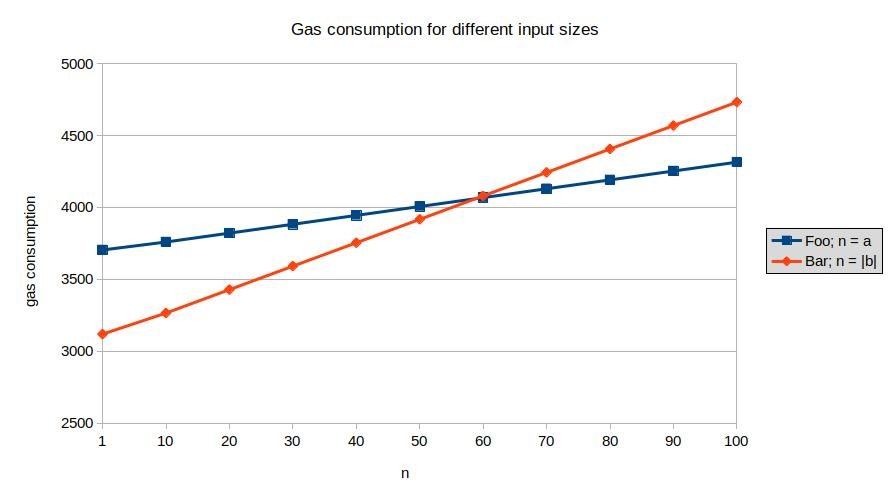
\includegraphics[width=0.9\linewidth]{figures/2-use_cases/cost_analysis}
\caption{Gas consumption of transactions calling \texttt{Foo} and \texttt{Bar} for increasing input sizes}
\label{fig:use_case_cost}
%\vspace{128in}
\end{figure}

Besides inflicting higher transaction costs on the user with increasing parameter sizes, a local approach also causes a higher ``footprint'' on the blockchain network. The transaction has to be processed at every full node of the network, which do not get any rewards in return (except for the nodes that were assigned baking or endorsement rights for the current block\footnote{Tezos' Proof of Stake consensus mechanism is described in \secref{sec:tezos}}).

    \externaldocument{1-introduction}

\chapter{Generic Offline Design}\label{chap:offline}
The implementation of distributed assertion checking on any blockchain requires some off-chain considerations and infrastructure. The previous chapter defined a formal set of logical formulae amenable for this approach and gave some in-depth examples. As stated before, the proposed implementation in the following chapters is, for the most part, restricted to formulas of predicate logic using universal quantification.\\
The purpose of the offline infrastructure is to provide a syntax for stating assertions that check logical formulas, as well as a toolchain to compile these assertions into code that can be originated on the target blockchain. Depending on the individual solution for the respective blockchain protocol, this can either be the original contract extended directly with the assertion code, or as a separate contract that extends the original contract in some other way. This chapter describes the generic part of the offline design, which corresponds to the front-end of the compilation pipeline shown in \figref{fig:pipeline_frontend}. As a start, \secref{sec:syntax} describes the concrete syntax for writing assertions and shows how it expresses some of the previously given examples. The transformation of the original assertions to assertions that check for counterexamples is formalized in \secref{sec:transformation}. Lastly, \secref{sec:accuracy} analyses the reliability of distributed assertion checking as proposed and the cost incurred by increasing it.

\begin{figure}[h]
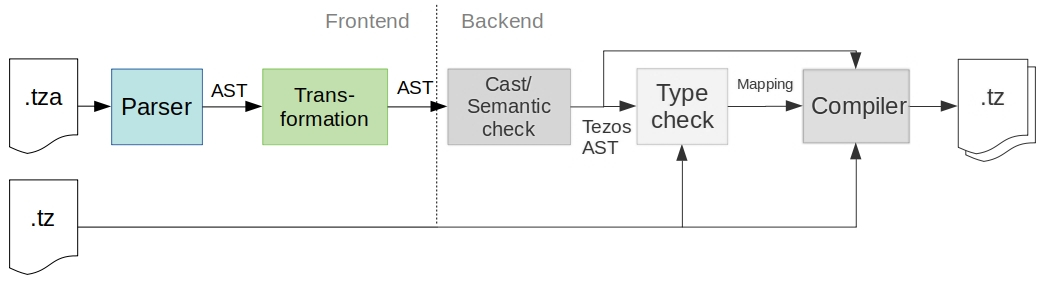
\includegraphics[width=\linewidth]{figures/3-offline/pipeline_frontend}
\caption{The stages of the generic frontend of the compilation pipeline}
\label{fig:pipeline_frontend}
\end{figure}

\section{Assertion syntax}\label{sec:syntax}
The assertion syntax is described in two versions by the EBNF grammars shown in appendix \ref{apx:grammar}. One version implements a prefix and the other one an infix notation. The pipeline currently supports the prefix notation with mandatory parentheses to avoid the need of handling operator precedences. To avoid context switches (at least for developers on Tezos), the assertion syntax references those of OCaml and thereby also Michelson.\\
A file containing assertions (henceforth referred to as ``assertion contract'') contains at least one assertion for some function or entrypoint of the original contract (henceforth referred to as ``parent contract''). An assertion begins with a signature consisting of an optional tag followed by a parameter type declaration. The tag can be used for documentation, but may sometimes be needed to indicate to which function of the parent contract the assertion should be assigned. The body is an (optional) nesting of quantifiers and conditions around exactly one assertion. Conditionals can be used to restrict the quantification domains or for some other constraints. For completeness, the existential quantifier is already included in the grammar, however the current version of the pipeline will reject any assertions containing it. \\
In order to make the front-end generic, the assertion grammar constitutes a union of operations and types for the target languages. This also allows the transformation to be oblivious of the target platform and be identical for all backends. The current version of the grammar recognizes all types present in the Tezos VM and a subset of operations that Michelson provides ( \secref{sec:tezos} contains an introduction to Tezos and Michelson and goes more into detail about this). Responsible for rejecting any assertions containing unsupported types or operations are the respective backends.\\

As an example, consider a variation of the formula given in \eqref{eq:sorted} that checks whether a given list is sorted in ascending order:
\begin{equation}\label{eq:sorted_v2}
	(\forall n : int)(\forall m : int) (0 \leq n < m < |a|) \Rightarrow a[n] \leq a[m]
\end{equation}
The respective assertion that checks this property for the parent contract from \lstref{lst:sorted} could be expressed as follows:
\lstinputlisting[caption=Assertion contract for checking if a list is sorted, language=Assertion, label={lst:sorted_assertion}]{listings/sorted.tza}

\subsection{Extensions}
In future iterations, the assertion syntax could be extended with some more features to improve usability and readability:
\begin{itemize}
\item \textbf{Local variables} to store, reuse and denominate computed values
\item \textbf{User-defined functions} to extract whole routines that can be reused in a single or even many assertion contracts, if defined as a module.
\item \textbf{if-else conditions} to adapt the domains of quantifications if certain conditions hold. The assertion that checks whether two numbers are relatively prime (discussed in \secref{sec:coprime}) is a good use-case for this feature: Firstly, the minimum of the given number has to be determined, however the \texttt{min}-function might not be supported as a built-in function by the target language (Tezos, for instance, does not support it). A solution for that could be to implement two branches in the program to handle each case. Secondly, if the greater of the two numbers is not evenly divided by the smaller one, the formula can be optimized by reducing the quantification domain by half to $(2 \le n \le \lfloor \frac{min(a,b)}{2} \rfloor)$, as a number cannot be evenly divided by any number between itself and its half \cite{bernhardt_veigel_2020}. With a syntax supporting an \texttt{if-else} control structure, the optimized assertion could look as follows:
\lstinputlisting[caption=Assertion syntax with if-else structures \cite{bernhardt_veigel_2020}, language=Assertion, label={lst:coprime}]{listings/coprime_ifelse.tza}
This feature is not included in the current version, because conditional domain restrictions make the translation from quantifiers to random generators or loops more complex. Aside from that, without the feature of variables and user-defined functions, the code is inflated significantly, thus causing increased origination cost.
\end{itemize}

\section{Transformation}\label{sec:transformation}
Since the validators will check the input parameter for the negation of the formula, it has to be transformed before compilation. Furthermore, the formula should explicitly state the domain for each quantifier, which will have to be translated into a set of bounds that refer to the respective random generator. Restricting the ranges of the random generators is important in order to avoid wasting resources through testing values out of the relevant (or legal) scope.

\subsection{Negation}
The formula is negated using the negation rules of second-order logic and applying De Morgan's laws \cite{de_morgan} until the negation is applied to the literals. Negating universal quantification is equivalent to an existential quantification of its negated body (and vice versa): $\neg \forall x P(x) \equiv \exists x \neg P(x)$ \cite{Sundstrom2020Quantifiers}. The domain restrictions are not affected by the negation, which is also reflected in the rules of predicate logic if the domain is given as a premise in the logical formula: $\neg (p \Rightarrow q) \equiv p \Rightarrow \neg q $.

\subsection{Building smart random generators}
In order to assign each explicit bound to its appropriate quantifier, the formula has be skimmed for atomic constraints that contain predicate (bound) variables. They're then moved and assigned to the quantifier that bounds the variable. If the constraint contains more than one bound variable, it is assigned to the quantifier with the highest depth in the order of quantifiers, as they depend on the generated value(s) of the other variable(s). \\
Revisiting the formula from \eqref{eq:sorted_v2}, its premise can be considered as a conjunction of the four constraints
\begin{itemize}
\itemsep-1em
\item $0 \leq n$
\item $n < |a| $
\item $n \le m$ and
\item $m < |a|$.
\end{itemize}
Applying the rules given above after negating the formula, the constraints are assigned to the quantifiers as follows:
\begin{equation}\label{eq:sorted_v2_bounds}
	(\exists n : int, 0 \leq n \wedge n < |a|])(\exists m : int, m > n \wedge m < |a|) \text{ } a[n] > a[m]
\end{equation}
Ultimately, the quantifiers are then translated to the corresponding random generators as indicated in \lstref{lst:rand}.
\begin{lstlisting}[label=lst:rand]
n = random(0, size(list))
m = random(n, size(list))
\end{lstlisting}
While conjunctions can be handled easily, other operators make it more difficult to derive efficient random generators. Consider the following constraints:
\begin{itemize}
\itemsep-0.7em
\item[1)] $(\forall n : int) (n < 10 \lor n > 20) ...$
\item[2)] $(\forall n : int) (n \ne 10) ...$
\item[3)] $(\forall n : int) (n = 10) ...$
\end{itemize}
Constraint 1) complicates restricting the random generator in several ways. Firstly, it separates the domain into two disjoint sub-domains, which requires defining a random generator for each range and another one to decide which one is called. Secondly, the operands of a disjunction cannot be considered separately when more than one bound variable is involved. For the predicate variable whose random generator is executed first, the domain restriction is optional, while the generation of the following random values depend on the previous result. Similarly to 1), constraint 2) splits the domain into sub-domains. To keep it simple for the time being, restrictions formulated with these operators are kept as part of the assertion code rather than used as constraints for the generators. Consequently, some validators may generate irrelevant values when checking the assertion and, depending on the size of the gap between the sub-domains, this can significantly decrease the reliability of this kind of assertion checking. Thus, further developed iterations should handle and translate them accordingly.\\
Constraint 3) effectively makes the quantifier, which binds $n$, obsolete. Adding this constraint to the respective generator will at least not affect the reliability, but a future improvement could be to optimize the assertion by replacing all occurrences of the bound variable with the assigned value and removing the quantification.

\subsection{Implicit constraints}
In some cases, boundaries are imposed implicitly by data types. List indices, for instance, are always bound to the range $0.. size(list) - 1$ and could thus be derived from the formula without an explicit specification. As this deduction makes the transformation more complex, requiring a semantic analysis of the formula, a completely explicit formula in terms of the domain is required for now. Depending on the VM, the lower bound for indexing operations can be implicitly handled by the random generator of an appropriate predicate type. As an example, Michelson supports the data type \texttt{nat} representing the natural numbers, which categorically excludes all values below zero. Developers aware of this can exploit this and, for instance, abbreviate \eqref{eq:sorted_v2} with the following formula:
\begin{equation}\label{eq:sorted_v2_abbr}
	(\forall n : nat)(\forall m : nat) (n \le m < |a|) \Rightarrow a[n] \leq a[m]
\end{equation}

\section{Accuracy of the approach}\label{sec:accuracy}
Since the proposed approach implements a probabilistic test, the accuracy as well as the costs incurred by guaranteeing a specified certainty threshold, need to be examined closely. The goal is to identify a formula that, given the domain of a formula in predicate logic, returns an estimate of a lower bound of samples necessary to find an existing counterexample with a probability $p$. From this analysis, it can be derived how effective a formula can be checked on a blockchain with $m$ validators. Sections \ref{sec:coupon} and \ref{sec:prob_threshold} depict the findings from \cite{bernhardt_veigel_2020} and are based on the assumptions that the random generator picks elements independently from a uniform distribution and that there exists exactly one counterexample for the passed parameter.

\subsection{Coupon Collector's Problem Analysis}\label{sec:coupon}
When checking properties with probabilistic testing, the result is either definitely not satisfied, or probably satisfied. Thus, errors only occur as false positives. In order to find an existing counterexample with probability $p = 1$, every element in the given domain $\mathcal{D}$ has to be checked by at least one validator. Deterministically, this is reachable with exactly $|\mathcal{D}|$ test runs. This is, however, invalid for the probabilistic approach, as some validators may generate duplicate random values and leave some elements of $\mathcal{D}$ unchecked. \\
In probability theory, this is known as the Coupon Collector's Problem \cite{croucher_collecting_2006}. Given $n = |\mathcal{D}|$, the probability that no duplicate elements are generated with $n$ picks is given by
\begin{equation*}
    p = \prod_{i=1}^{n} \frac{i}{n}
\end{equation*}
As an example, the probability that all validators generate a unique random value already drops to $0.036\%$ for $n = 10$. Let the random variable $T$ be the number of test runs executed until every element in the domain has been generated. In order to obtain an estimation of how many test runs are needed to find the counterexample for certain, the goal is to identify its expectation $E(T)$. To this end, the geometric probability distribution is applied \cite{croucher_collecting_2006}:\\
Each element is generated with a probability of $1/n$. Thus, the probability to generate the $i$th unique element is given by 
\begin{equation}
    p_i = \frac{n-i+1}{n}
\end{equation}
\cite{croucher_collecting_2006}. The expected value of a random variable $X$ is given by $E(X) = \frac{1}{p}$\cite{croucher_collecting_2006}, thus the expected number of test runs for $n$ is 
\begin{equation}
E(T) = n \sum_{i=1}^{n} \frac{1}{i}
\end{equation}
\tabref{tab:prob_outcomes} shows the expected number of test runs $E(T)$ and its standard deviation $\sigma$ for different $n$. Furthermore, $E(T)$ and $\sigma$ are used to calculate a 95\% confidence interval for $T$ by applying the central limit theorem, which provides an upper and lower bound on the number of test runs \cite{croucher_collecting_2006}. Rounded values for both bounds are also shown in \tabref{tab:prob_outcomes}.
\begin{table}[h]
    \centering
    \begin{tabular}{lllll}
        \thead{$n$} & \thead{$E(T)$} & \thead{$\sigma$} & \thead{lower bound} & \thead{upper bound}\\ \hline
        5 & 11.4 & 2.53 & 6 & 16\\
        10 & 29.3 & 4.32 & 21 & 38\\
        20 & 72.0 & 7.21 & 58 & 86\\
        30 & 119.8 & 9.48 & 101 & 138 \\
        50 & 225.0 & 13.23 & 199 & 251 
    \end{tabular}
    \caption{Expectation, standard deviation and upper and lower bound of needed test runs for some $n$ \cite{croucher_collecting_2006}}
    \label{tab:prob_outcomes}
\end{table}

The results show that checking random values is a very inefficient approach if false positives are not admissible. Even if the lower bound of $T$ is chosen as the number of test runs, it exceeds the size of the domain by far and increases the time complexity to $\mathcal{O}(n*log(n))$ for large $n$ \cite{xu_tang_2011}. For instances where false positives are tolerable, the following section introduces a formula to calculate the number of test runs that detect counterexamples with a given probability threshold $p \leq 1$.

\subsection{Setting probability thresholds}\label{sec:prob_threshold}
The goal is to find a number $t$ of test runs, s.t. the probability $P_{c,t}$ of not finding the counterexample drops below a certain threshold $c$. A validator finds the counterexample in one test run with probability $\frac{1}{n}$, and misses it with probability $(1-\frac{1}{n})$. After $t$ tests runs, the probability that the counterexample has not been found is thus $(1-\frac{1}{n})^t$. Following the same approach as in \cite{mahl_schindel_2007} to retrieve an upper bound for $P_{c,t}$, we use the following inequality
\begin{equation}
(1-\frac{1}{m})^m \leq \frac{1}{e}
\end{equation}
which holds for all $m > 0$. From this inequality, it follows that
\begin{equation}
(1-\frac{1}{n})^t = ((1-\frac{1}{n})^n)^{\frac{t}{n}} \le e^{-\frac{t}{n}}
\end{equation}
With this, the probability $P_{c,t}$ of not finding the counterexample with $t$ test runs can be defined as
\begin{equation}
P_{c,t} \le e^{-\frac{t}{n}}
\end{equation}
In order to retrieve the number of test runs $t$ necessary for $P_{c,t}$ to drop below a specified threshold $c$, the inequality is solved for $t$, which is then dependent of the known parameter $n$ and an arbitrary value for $c$:
\begin{align}
    e^{-\frac{t}{n}} &\leq c && \text{with } 0 \leq c\le 1 \nonumber\\
    t &\geq -n\:\ln(c)
\end{align}
For $c = \frac{1}{e}$ ($\approx 36.79\:\%$) the lower bound of $t$ is exactly $n$, which means that for higher reliabilities the number of test runs needs to be greater than $n$. \figref{fig:graph_t_c} shows the lower bounds of $t$ as a function of the probability threshold and domain size. One can see that the increase in accuracy is approximately linear to the number of test runs below a threshold of $c=0.5$, but requires an exponential testing effort to reach higher thresholds.
\begin{figure}[h]
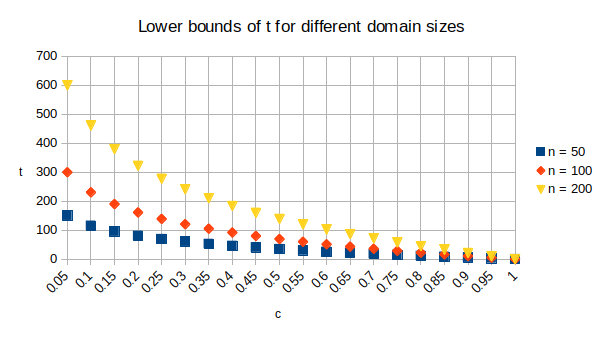
\includegraphics[width=0.95\linewidth]{figures/3-offline/graph_t_c}
\caption{The number of required test runs as a function of the probability of false positives $c$ and size of the domain $n$}
\label{fig:graph_t_c}
\end{figure}
For assertions with several quantifiers, which are translated to random generators, all domains have to be considered in the calculation. Revisiting the intersection of sets from \secref{sec:existential}, every element in set $U$ has to be compared to every element in set $V$. Thus, the lower bound of test runs needed to check whether they intersect with a certainty of 63.21\% is given by $t \leq t_1 * t_2$ with $t_1 \geq |U|$ and $t_2 \geq |V|$.

\subsection{Validators vs. test runs}
The last section derived a formula to calculate a lower bound for a number of test runs $t$ in order to reach a certain level of confidence. However, $t$ is not a parameter that can be adjusted to an arbitrary value on the blockchain, as the assertion is checked by the validators. Assuming a blockchain has $m$ validators, the actual lower bound of test runs is $m$. For cases where there are not enough validators to reach a threshold $c$, a mechanism is required to have each validator check the property for multiple random values. Hence, the actual executed number of checks is always a multiple of $m$. \secref{} goes into a bit more detail about this based on the Tezos blockchain. \todo{Refer to section}

\subsection{Alternatives to random testing}
For applications where higher reliability is crucial, an alternative to checking elements randomly could be to coordinate a systematic iteration of the domain. The implementation of such a coordination is not trivial though; validators can't simply be passed an individual value as input. Instead, possible approaches could be to implement a central instance that allocates an element in the search space to each validator, or use some unique and intrinsic attribute, like an identification number, as input for a mapping. The discussion if this approach would provide any advantages over a local validation of the property is left open \todo{Depends on cost analysis?}.

\subsubsection{Central instance assigning values}
For this approach, the tool-chain would need to generate a separate contract that is called by the miners and validators as a proxy. This contract would then, for instance, generate a number using a modulo-n counter and pass this number as an additional parameter to the assertion code. The random generators would be omitted accordingly. However, this works only as expected if there are no simultaneous transactions calling the contract, otherwise it cannot be guaranteed that all elements have been checked for each of the transactions. If and how this issue can be solved will not be discussed further in this thesis.

\subsubsection{Using unique attributes of a validator}\label{sec:alt_attributes}
This approach strongly depends on whether the validators have a unique id or other attribute that can be accessed from within a contract.  If there is (or the language can be extended with such a feature), there needs to exist a non-injective surjective function that maps the respective attributes represented by type A to an element of the domain represented by type B, i.e. $f: X \rightarrow Y$. Furthermore, for cases where $t > m$, an offset needs to be added, s.t. a validator checks distinct elements for each test run. \\
Implementing such an approach on Tezos becomes even more challenging due the way endorsing (i.e. validation) rights are distributed in its proof-of-stake mechanism: for each block level, endorsing rights are assigned to the owner of a randomly selected roll, i.e., a set of tokens \cite{tezos_docs}. This means that the same validator can be picked multiple times for endorsing one block and thus some elements in the domain may remain unchecked. \secref{} goes into more detail about this issue. \todo{Ref section}
    \chapter{Probabilistic model}\label{chap:prob_model}
Since the proposed approach implements a probabilistic validation, the reliability of the result depends on the number of validators in the network in relation to the size of the iteration space. Given that the number of validators is finite, the probability of finding existing counterexamples may drop below an acceptable threshold for higher domain sizes. Thus, the distributed assertion checking scheme should provide a mechanism to have each validator invoke the assertion contract a specified number of times. To this end, it is necessary to identify a formula which, given the domain size and a probability threshold, returns a lower bound for the required number of test runs per validator. 

Sections \ref{sec:coupon} and \ref{sec:prob_threshold} describe the findings from a collaborative work with Julian Veigl \cite{bernhardt_veigel_2020}. They are based on the assumption that random generators pick elements independently from a uniform distribution. Furthermore, all calculations are based on the worst case scenario, in which there exists exactly one counterexample for the given input.

\section{Sample spaces}
The sample space of an assertion in form of a logical formula is given by the domains of discourse of the quantifiers. \secref described, that the premises defining the domains are translated into a list range constraints of the random generators. Based on these constraints, the compiler can derive a formula to determine the size of the sample space at runtime. In simple cases, the sample space is given by a single domain. Such a space is given, for instance, in the introductory example checking whether a number is a prime, i.e., $\mathcal{S} = \lbrace n \in\mathbb{Z} : 2 \le n \le \sqrt{p} \rbrace$. Based on the constraints $2 \le n$ and $n \le \sqrt{p}$, the size of the search space can be determined at runtime with $|\mathcal{S}| = \sqrt{p} - 2$. If the assertion has to sample from more than one domain, the search space is given by the Cartesian product of these domains, or sub-search spaces. In the example of intersecting sets from \secref{sec:existential}, the sample space is $\mathcal{S} = \mathcal{S}_U \times \mathcal{S}_V$, where $\mathcal{S}_U = \lbrace n \in\mathbb{Z} : 0 \leq n \le |U| \rbrace$ (analogue for $\mathcal{S}_V$). At runtime, the size of the search space can be determined with $|\mathcal{S}| = (|U| - 0) + (|V| - 0)$.

\section{Coupon Collector's Problem Analysis}\label{sec:coupon}
When checking properties with probabilistic testing, the result is either definitely not satisfied, or probably satisfied. Thus, errors only occur as false positives. In order to find a counterexample with probability $p = 1$, every element in the given search space $\mathcal{S}$ has to be checked by at least one validator. Deterministically, this is reachable with exactly $|\mathcal{S}|$ test runs. This is, however, invalid for the probabilistic approach, as some validators may generate duplicate random values and leave some elements of $\mathcal{S}$ unchecked. \\
In probability theory, this is known as the Coupon Collector's Problem \cite{croucher_collecting_2006}. Given $n = |\mathcal{S}|$, the probability that no duplicate elements are generated with $n$ picks is given by
\begin{equation*}
    p = \prod_{i=1}^{n} \frac{i}{n}
\end{equation*}
As an example, the probability that all validators generate a unique random value already drops to $0.036\%$ for $n = 10$. Let the random variable $T$ be the number of test runs executed until every element in the search space has been generated. In order to obtain an estimation of how many test runs are needed to find the counterexample for certain, the goal is to identify its expectation $E(T)$. To this end, the geometric probability distribution is applied \cite{croucher_collecting_2006}:\\
Each element is generated with a probability of $1/n$. Thus, the probability to generate the $i$th unique element is given by 
\begin{equation}
    p_i = \frac{n-i+1}{n}
\end{equation}
\cite{croucher_collecting_2006}. The expected value of a random variable $X$ is given by $E(X) = \frac{1}{p}$\cite{croucher_collecting_2006}, thus the expected number of test runs for $n$ is 
\begin{equation}
E(T) = n \sum_{i=1}^{n} \frac{1}{i}
\end{equation}
\tabref{tab:prob_outcomes} shows the expected number of test runs $E(T)$ and its standard deviation $\sigma$ for different $n$. Furthermore, $E(T)$ and $\sigma$ are used to calculate a 95\% confidence interval for $T$ by applying the central limit theorem, which provides an upper and lower bound on the number of test runs \cite{croucher_collecting_2006}. Rounded values for both bounds are also shown in \tabref{tab:prob_outcomes}.
\begin{table}[h]
    \centering
    \begin{tabular}{lllll}
        \thead{$n$} & \thead{$E(T)$} & \thead{$\sigma$} & \thead{lower bound} & \thead{upper bound}\\ \hline
        5 & 11.4 & 2.53 & 6 & 16\\
        10 & 29.3 & 4.32 & 21 & 38\\
        20 & 72.0 & 7.21 & 58 & 86\\
        30 & 119.8 & 9.48 & 101 & 138 \\
        50 & 225.0 & 13.23 & 199 & 251 
    \end{tabular}
    \caption{Expectation, standard deviation and upper and lower bound of needed test runs for some $n$ \cite{croucher_collecting_2006}}
    \label{tab:prob_outcomes}
\end{table}

The results show that checking random values is a very inefficient approach if false positives are not admissible. Even if the lower bound of $T$ is chosen as the number of test runs, it exceeds the size of the search space by far and increases the time complexity to $\mathcal{O}(n*log(n))$ for large $n$ \cite{xu_tang_2011}. For instances where false positives are tolerable, the following section introduces a formula to calculate the number of test runs that detect counterexamples with a given probability threshold $p \leq 1$.

\section{Setting probability thresholds}\label{sec:prob_threshold}
The goal is to find a number $t$ of test runs, s.t. the probability $P_{c,t}$ of not finding the counterexample drops below a certain threshold $c$. A validator finds the counterexample in one test run with probability $\frac{1}{n}$, and misses it with probability $(1-\frac{1}{n})$. After $t$ tests runs, the probability that the counterexample has not been found is thus $(1-\frac{1}{n})^t$. Following the same approach as in \cite{mahl_schindel_2007} to retrieve an upper bound for $P_{c,t}$, we use the following inequality
\begin{equation}
(1-\frac{1}{m})^m \leq \frac{1}{e}
\end{equation}
which holds for all $m > 0$. From this inequality, it follows that
\begin{equation}
(1-\frac{1}{n})^t = ((1-\frac{1}{n})^n)^{\frac{t}{n}} \le e^{-\frac{t}{n}}
\end{equation}
With this, the probability $P_{c,t}$ of not finding the counterexample with $t$ test runs can be defined as
\begin{equation}
P_{c,t} \le e^{-\frac{t}{n}}
\end{equation}
In order to retrieve the number of test runs $t$ necessary for $P_{c,t}$ to drop below a specified threshold $c$, the inequality is solved for $t$, which is then dependent of the known parameter $n$ and an arbitrary value for $c$:
\begin{align}
    e^{-\frac{t}{n}} &\leq c && \text{with } 0 \leq c\le 1 \nonumber\\
    t &\geq -n\:\ln(c)
\end{align}
For $c = \frac{1}{e}$ ($\approx 36.79\:\%$) the lower bound of $t$ is exactly $n$, which means that for higher reliabilities the number of test runs needs to be greater than $n$. \figref{fig:graph_t_c} shows the lower bounds of $t$ as a function of the probability threshold and search space size. One can see that the increase in accuracy is approximately linear to the number of test runs below a threshold of $c=0.5$, but requires an exponential testing effort to reach higher thresholds.
\begin{figure}[h]
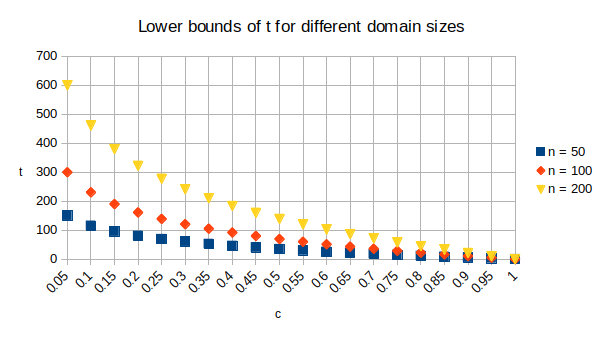
\includegraphics[width=0.95\linewidth]{figures/3-offline/graph_t_c}
\caption{The number of required test runs as a function of the probability of false positives $c$ and size of the search space $n$}
\label{fig:graph_t_c}
\end{figure}

\section{Validators vs. test runs}
The last section derived a formula to calculate a lower bound for a number of test runs $t$ in order to reach a certain level of confidence. However, $t$ is not a parameter that can be adjusted to an arbitrary value on the blockchain, as the assertion is checked by the validators. Assuming a blockchain has $m$ validators, the actual lower bound of test runs is $m$. For cases where there are not enough validators to reach a threshold $c$, a mechanism is required to have each validator check the property for multiple random values. Hence, the actual executed number of checks is always a multiple of $m$.

\section{Alternatives to random testing}\label{sec:alt_random}
For applications where higher reliability is crucial, an alternative to checking elements randomly could be to coordinate a systematic iteration of the domain. The implementation of such a coordination is not trivial though; validators can't simply be passed an individual value as input. Instead, possible approaches could be to implement a central instance that allocates an element in the search space to each validator, or use some unique and intrinsic attribute, like an identification number, as input for a mapping.

\subsection{Central instance assigning values}
For this approach, the tool-chain would need to generate a separate contract that is called by the miners and validators as a proxy. This contract would then, for instance, generate a number using a modulo-n counter and pass this number as an additional parameter to the assertion code. The random generators would be omitted accordingly. However, this works only as expected if there are no simultaneous transactions calling the contract, otherwise it cannot be guaranteed that all elements have been checked for each of the transactions. If and how this issue can be solved will not be discussed further in this thesis. Another drawback of this approach is that it leads to a serialization of the tests, as the contract has to update its internal storage.

\subsection{Using unique attributes of a validator}\label{sec:alt_attributes}
This approach strongly depends on whether the validators have a unique id or other attribute that can be accessed from within a contract.  If there is (or the language can be extended with such a feature), there needs to exist a non-injective surjective function that maps the respective attributes represented by type A to an element in the search space, represented by type B, i.e. $f: X \rightarrow Y$. Furthermore, for cases where $t > m$, an offset needs to be added, s.t. a validator checks distinct elements for each test run. \\
Implementing such an approach on Tezos becomes even more challenging due the way endorsing (i.e. validation) rights are distributed in its proof-of-stake mechanism: for each block level, endorsing rights are assigned to the owner of a randomly selected roll, i.e., a set of tokens \cite{tezos_docs}. This means that the same validator can be picked multiple times for endorsing one block and thus some elements in the search space may remain unchecked. \secref{} goes into more detail about this issue. \todo{Ref section}
    \chapter{Toolchain Backend}\label{chap:offline_tezos}
After parsing and transforming a list of assertions, the resulting ASTs are passed to the target-specific backend. For this thesis, the platform target is Tezos, with Michelson as the compilation target. The pipeline stages of the backend comprise the ones colourized in \figref{fig:pipeline_backend}. First, the generic ASTs are subjected to a semantic check, which rejects any assertions containing unsupported types, operations or other invalid expressions. Valid ASTs are then cast to a target specific AST type and passed to the type checker. In this stage, the assertions are linked to the respective parent entrypoints, based on the parameter patterns and tags. Given the list of target specific ASTs and a linking, the compiler finally generates target code. Each stage is described in more detail in \secref{sec:backend_impl}.

As a preliminary and preparation for the compiler implementation, \secref{sec:ext_michelson} identifies necessary extensions to Michelson and Tezos' VM, in order to facilitate the distributed assertion scheme. Although the extensions are formalized in this thesis, implementing the extension is part of the protocol amendment. Furthermore, the compiler needs to generate the target code according to an on-chain orchestration scheme between the assertion and parent contract. This orchestration includes the mechanism to trigger several assertion checks per validator based on \eqref{eq:test_runs}, which was derived in the previous chapter. \secref{sec:orchestration} explores possible strategies for such a scheme, and discusses their strengths and weaknesses. Based on a resulting proposal for the orchestration, \secref{sec:cost_analysis_distributed} performs a cost analysis of distributed assertion checking and evaluates if, and under which conditions, it can increase the scalability in blockchain applications.

As a foundation for the other sections, \secref{sec:tezos} provides important background on the Tezos blockchain, its built-in smart contract language Michelson and some relevant tools and projects within its ecosystem.

\section{Tezos}\label{sec:tezos}
The Tezos blockchain is presented in its whitepaper as a \enquote{generic and self-amending crypto-ledger} \cite{goodman_tezos_2014}. It uses a proof-of-stake consensus mechanism, which is not only used to agree on the current state of its ledger, but also allows its stakeholders to come to a consensus about changes in the economic protocol by participating in a voting process. The changes included in a protocol upgrade, called amendment, can influence, i.a., which transactions are valid on the blockchain, the payment system or even the voting process itself. It does so without risking a fork of the blockchain. Everyone owning the cryptocurrency of Tezos, called Tez, is considered a stakeholder and can participate in the consensus mechanism. The whitepaper compares the self-amending protocol of Tezos to a game created by Philosopher Peter Suber called ``Nomic'', whose set of rules are subjected to a democratic voting system \cite{nomic}. Similar concepts can also be found in modern pop culture, such as the virtual sports league ``Blaseball'' \cite{blaseball}, which became popular during the COVID-19 pandemic.

In addition to user accounts associated with a public key, Tezos supports smart contracts, which are written in the built-in language Michelson. Tezos' transaction fee system is similar to Ethereum's \cite{wood_ethereum_2021} - it is gas-instrumented and besides a base fee, every operation and byte of storage during contract execution has to be paid for by the user. However, Tezos imposes a hard cap on the amount of gas that can be consumed per operation (including internal transactions) \cite{tezos_docs}\cite{morley_repo}, whereas Ethereum limits the gas quota only in respect to blocks \cite{wood_ethereum_2021}.\\
Tezos is written in the multi-paradigm programming language OCaml. Compiling its source code yields five essential binaries: the  node, baker, endorser, accuser and client. The node is the entity connecting to the peer-to-peer network and keeping a copy of the chain. Bakers are responsible for producing new blocks, the endorsers for validating new blocks and the accusers to call out bakers or endorsers which double-sign or -endorse. The client provides a command line interface to interact with nodes through remote procedure calls (RPC). 

\subsection{Proof-of-stake in Tezos}
In Tezos, contracts which have staked a minimum amount of tokens (called a roll), can participate in the consensus mechanism. When participating, a contract has a chance to obtain the role of either a baker or an endorser. Contracts not owning enough tokens or infrastructure to participate directly, can delegate their baking and endorsing rights to other contracts. The rights to bake or endorse are determined and assigned at the beginning of each cycle, which consists of a specified number of blocks. For baking, a random roll is selected for each block level and the rights are assigned to its owner. The block produced by that baker is signed by a fixed number of endorsers\footnote{For consistency, endorsers are referred to as ``validators'' in the remainder of this chapter} (32 as of protocol 007 Delphi), which also have been assigned endorsing rights for this block level by a random selection of rolls. Since participants can stake more than one roll, they may be assigned several endorsement slots at the same block level.

As an incentive for active participation in the consensus algorithm, delegates (and also delegators) receive rewards in form of tokens. However, if accusers detect double-baking or -endorsement, the delegate is penalized by burning (i.e., destroying) their security deposit.

\subsection{Michelson}
Michelson is a lower-level, stack-based language with strict type-checking. It supports primitive data types, like integers or strings, as well as high-level data structures, such as list, maps and sum types. The type system reduces the occurrence of runtime errors and ensures that only well-typed contracts are originated on the blockchain.

The concrete syntax of Michelson is called Micheline. A program is represented as Micheline nodes, which can be one of the following constructs:
\begin{itemize}
\item A constant of type integer (in decimal notation)
\item A constant of type string
\item A byte sequence in hexadecimal notation
\item An application of a language primitive to a sequence of nodes
\item A sequence of nodes
\end{itemize}
For documentation, readability and additional type constraints, Michelson and Micheline also offer three types of annotations - type, variable and field or constructor annotations, which are labelled with a unique special character in Micheline. The toplevel structure of a smart contract consists of a sequence of the three primitives \texttt{parameter, storage} and \texttt{code}. They declare the type of the input parameter, the storage type and the script, which is interpreted when the contract is invoked. The full grammar of Micheline and Michelson can be found in the Tezos developer resources \cite{tezos_docs}.

\subsubsection{Entrypoints}
Unlike Ethereum's contract language Solidity, Michelson doesn't have a concept of named functions with a dedicated parameter type. Instead of named functions, Michelson contracts model separate entrypoints by taking a sum type as an input parameter. The type constructors can optionally be tagged with a field annotation, which can be considered  as an entrypoint name. The sum type is built by nesting the \texttt{or} data type, which has the constructors \texttt{left} and \texttt{right}. As an example, the contract in \lstref{lst:entrypoints} has two entrypoints --- entrypoint \texttt{A}, which expects an integer wrapped in the \texttt{left} constructor, e.g. \texttt{left 1}, and entrypoint \texttt{B}, which expects a string wrapped in the \texttt{right} constructor, e.g. \texttt{right "hello world"}.
\begin{lstlisting}[language=Michelson, numbers=none, caption=Michelson contract with two entrypoints, label=lst:entrypoints]
parameter (or (int %A) (string %B));
storage unit;
code {
  ...
  IF_LEFT { ... (* entrypoint A *)}
          { ... (* entrypoint B *)}
}
\end{lstlisting}
By adding the constructor annotations \texttt{A} and \texttt{B}, the entrypoints can be invoked explicitly. The passed parameter value is then wrapped automatically into the respective constructor. Furthermore, it is possible to declare a \texttt{default} entrypoint, which is invoked when no explicit tag is specified in the transaction. By default, the default entrypoint is assigned to the root of the parameter type.

\subsubsection{Internal Operations}\label{sec:internal_ops}
Smart contracts are able to invoke other contracts by emitting internal operations. The return type of Michelson programs (more specifically, the type of the top element on the stack after the completed execution) is a tuple of a list of internal operations and the updated storage. After a contract completes, the operations in the returned list are run in sequence. Since internal operations may in turn also emit internal operations, the interpreter puts all emitted operations into a queue, which is processed in order. As an example, \figref{fig:internal_ops} shows an execution order of two external transactions and their internal operations in sequence.
\begin{figure}[h]
\centering
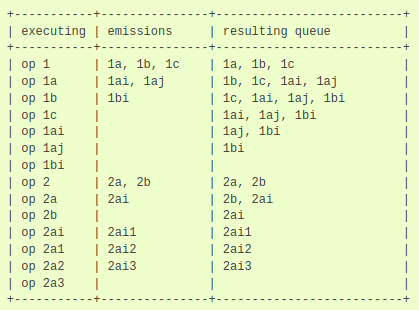
\includegraphics[width=0.5\linewidth]{figures/5-offline_tezos/internal_ops}
\captionsource{Execution order of two external operations and their internal operations}{\cite{tezos_docs}}
\label{fig:internal_ops}
\end{figure}

Both external and internal operations can fail, if the source contract does not have enough balance to spend the specified amount, a gas limit was reached, or if a program fails due to reaching a \texttt{FAILWITH} instruction. If a failure occurs, the whole sequence fails and all changes up to the point of failure are reverted. Within a sequence, an operation can thus have one of the following result types:
\begin{itemize}
\item \textbf{Applied} --- the operation was successful
\item \textbf{Failed} --- the operation failed
\item \textbf{Skipped} --- the operation was in sequence after a failed operation
\item \textbf{Backtracked} --- reverted operation due to a failed operation further along in the sequence
\end{itemize}

\subsection{Gas Model}
Tezos stores and transmits data as byte sequences --- in order to obtain a typed representation of their value for interpretation, a byte sequence is first deserialised into Micheline and subsequently parsed into a typed AST. Conversely, before transmitting or storing something on the blockchain, the typed representation is first unparsed into Micheline and then serialised. Since these working steps also entail computational effort, they consume gas and thus account for some of the transaction fees. The gas consumption of an operation (e.g., a transaction or a contract origination) is thus composed of the following positions on top of a base gas fee \cite{morley_gasmodel}\cite{tezos_repo}:
\begin{enumerate}
\item \textbf{Reading costs} --- apply for reading the contract code and storage from the blockchain and depend on the amount of bytes read
\item \textbf{Deserialization costs} --- depend on the components of the Micheline expression and the size of the byte sequence. Apply lazily, thus the deserialization of each value only has to be paid for once
\item \textbf{Parsing costs} --- are composed of three types of costs:
	\begin{itemize}
	\item type parsing --- apply when a Micheline node is converted into a valid type
	\item data parsing --- apply when a node is converted into the value of a known type and depends on the size of the value
	\item code parsing --- apply when the instructions of a program are type checked and depends on the number and types of instructions. Some instructions are expensive, such as \texttt{IF} (both branches need to be checked and compared) or \texttt{CREATE\_CONTRACT} (requires type check of the invoked contract)
	\end{itemize}
\item \textbf{Type comparison costs} --- apply when types are checked for equality (e.g. when type checking the branches of the \texttt{IF} instruction) or during contract interpretation
\item \textbf{Interpretation costs} --- apply for each interpreted instruction and depend on their computational complexity.
\item \textbf{Unparsing costs} --- apply when converting typed data to untyped Micheline nodes and depend on the data type and size
\item \textbf{Serialization costs} --- apply when serializing Micheline nodes to byte sequences and depend on the expression and its size
\item \textbf{Writing costs} --- apply when writing to the internal database and depend on the amount of bytes. A base gas fee is burned for each additional byte of storage.
\end{enumerate}
If a transaction emits internal operations, their gas consumption is computed in the same way and is added to the total gas consumption of the external operation.

\subsection{Developer Tools in the Tezos Ecosystem}
This section describes some tools and projects within Tezos' ecosystem, which are relevant to the development of the toolchain or the protocol amendment.

\subsubsection{Tezos Libraries}
Tezos' executables and libraries are available on OCaml's package manager \texttt{opam} \cite{tezos_opam}. The protocol libraries of every version are released separately, thus any projects can be built on the protocol of choice. Relevant libraries included in the backend of the toolchain are, i.a, the Micheline library containing the internal abstract syntax tree (AST) and parser of the Michelson language, the protocol libraries providing functions to type check code or data, and client libraries to retrieve any needed information from the node or blockchain via wrapped RPCs.

\subsubsection{Testing Tools}
Before a new protocol is proposed to the Tezos network, it has to be thoroughly tested with system, integration and regression tests. This requires a sandboxed network to simulate the real peer-to-peer network. Tezos' development environment provides the two testing frameworks Flextesa (Flexible network sandboxes)\cite{tezos_docs} and its successor Tezt \cite{tezos_docs}. They allow to configure and run a small, fully functional sandboxed test network including nodes, bakers, endorsers and accusers. Besides testing new protocols, they can also be used to interactively test smart contracts.

\subsubsection{High-level Languages}\label{sec:languages}
Michelson is a compilation target for various high-level languages that provide a more user-friendly and intuitive way of writing smart contracts. Additionally, some of them provide development environments, testing or verification tools. The following list introduces three prominent languages, which compile to Michelson:
\begin{description}
\item[\textbf{Liquidity}] \cite{liquidity} is a language with an OCaml-like syntax, which allows to express contracts in a functional way. It supports using local variables instead of stack manipulations. Its module system can be used to write reusable contract code or libraries. Besides an optimizing compiler, the project also includes a decompiler to compile Michelson programs to Liquidity source code.
\item[\textbf{SmartPy}] \cite{smartpy} is a language available through a Python library and lets developers write contracts and tests using Python syntax and structures (such as classes). Its developer suite includes, i.a., a compiler, a simulation engine for testing contracts and an online editor.
\item [\textbf{Ligo}] \cite{ligo} offers multiple syntax flavours close to Pascal, OCaml or Reason. Besides compilation, the toolchain allows to invoke or evaluate the generated code locally. The project provides Ligo as OCaml packages, which can be integrated into other projects.
\end{description}

\section{Extensions to Michelson}\label{sec:ext_michelson}
For the assertion code to be executable by the VM of Tezos, Michelson and the VM have to be extended with new instructions. This includes an instruction to generate a random value of some primitive data type non-deterministically. The formalization and possible implementation of such an instruction is described in \secref{sec:random}. Aside from this, many useful use-cases involve checking random elements of lists, and possibly strings or bytes. For convenience, it is worth considering adding indexing operations for some data types to the VM. This is discussed in more detail in \secref{sec:nth}.

As a foundation for the formalization of these new instructions, \secref{sec:michelson_semantics} gives a brief introduction to the Michelson interpreter and type system first.  

\subsection{Language Semantics and Type System}\label{sec:michelson_semantics}
Michelson is interpreted purely functional; the interpreter takes the current stack and an operation and builds a return stack from the initial one, without causing any side effects. The definition of the recursive interpreter is given in the form of a list of rules, comprising of all possible inputs (i.e., program and stack types) and the respective output stack type of the computation. Each rule is of the following form: 
\begin{lstlisting}[caption=Selection rules in the Michelson interpreter \cite{tezos_docs}, language=, numbers=none, label=lst:rules]
> (syntax pattern) / (initial stack pattern)  =>  (result stack pattern)
    iff (conditions)
    where (recursions)
    and (more recursions)
\end{lstlisting}
For each valid program and initial stack, exactly one rule applies. Following the keyword \texttt{iff}, the rule can add extra conditions over values on the stack. If the result depends on the results of other program interpretations, such as conditionals or function calls, the rule can contain recursive rules in the \texttt{where} or \texttt{and} clauses. These clauses represent a recursive interpretation of an intermediate program. The rule thus only applies, if the interpretation of the intermediate result matches the expected pattern.

The type system of Michelson consists of typing rules for each syntax construct, restricting the valid input stacks. The typing rules use the meta variables \texttt{'a} for type, and \texttt{'A} for stack type variables. Using these meta variables, the rules express consistency within the program. The typing rules are given in the form shown in \lstref{lst:type_rules}, where premises are additional typing requirements over values on the stack:
\begin{lstlisting}[caption=Form of typing rules in Michelson's specification \cite{tezos_docs}, language=, numbers=none, label=lst:type_rules]
(syntax pattern)
:: (type of stack before) -> (type of stack after) [rule-name]
   iff (premises)
\end{lstlisting}
The Tezos developer resources \cite{tezos_docs} provide a comprehensive list of type notations, syntax and stack patterns.

Since the Michelson language and interpreter are implemented in the protocol-specific libraries of Tezos, adding new instructions require a protocol update. This entails adding the new instruction to the list of tokens, adding one or several selection rules to the interpreter and typing rules to the type checker \cite{tezos_repo}. Furthermore, the protocol must specify the gas cost of its computation. Previous extensions to the Michelson language, such as the addition of the instruction ``\texttt{DIG n}'' in protocol 005 Babylon \cite{tezos_michelson_ext}, can be used as a guideline for the extension. The gas cost specification of existing instructions \cite{tezos_repo_gas} should be used as an orientation in specifying the costs of new instructions.

\subsection{Random Instruction}\label{sec:random}
Since smart contracts generally need to be deterministic, s.t. the network can reach a consensus about the state of the ledger \cite{chatterjee_probabilistic_2019}, the prevalent workarounds for generating pseudo-random numbers cannot be used to implement the random generators in assertion contracts. The scheme explicitly requires the validators to check distinct elements in the search space. Common schemes for obtaining random values, like oracles or using block attributes as seeds \cite{chatterjee_probabilistic_2019}, would generate the same values for all validators. Thus, the VM needs to provide an instruction to generate a ``real'' random value exclusively for assertion checking. In order to preserve the deterministic behaviour of normal smart contracts, the instruction should not be available in the normal execution mode.

\lstref{lst:rand_type} specifies the typing and selection rule of a new instruction \texttt{random} for integers, although such an instruction could also be provided for other data types, such as \texttt{nat}, \texttt{string} or \texttt{mutez}. The selection rule for this instruction applies for the instruction identifier \texttt{RANDOM} and an input stack containing at least two elements. It consumes an offset and a positive range from the stack and pushes a randomly generated integer to the top. The typing rule (line 1) specifies, that the offset should be of type \texttt{integer}, and the range of type \texttt{nat} (i.e., a natural number).
\lstset{upquote=true}
\begin{lstlisting}[caption=Typing and selection rules of the integer \texttt{random} instruction, language=, showlines=true, label=lst:rand_type]
:: int : nat: 'A -> int : 'A
> RANDOM / offset : range : S  => int : S
\end{lstlisting}

Within the Michelson interpreter, the selection of rules is implemented as a huge match case \cite{tezos_repo}. If the rule for \texttt{random} applies, the instruction could be computed in OCaml as indicated in \lstref{lst:rand_impl}.
\begin{lstlisting}[caption=Simplified evaluation of \texttt{random} in the Michelson interpreter, language=, label=lst:rand_impl, float]
match (instruction, stack) with
...
| (Random (offset, (range, rest))) ->
   Random.self_init;
   let rand_int = offset + Random.int(range) in
   return (rand_int, rest)  (* resulting stack *)
\end{lstlisting}

\subsection{List Indexing}\label{sec:nth}
Michelson currently does not provide any predefined indexed access operators for data types like lists, strings or bytes. Accessing a random element of a sequence can, of course, be implemented using low-level instructions. However, because such operations are used frequently in many of the given use-cases, adding it as a predefined primitive for some data types might be justifiable. It reduces the required code to express the indexing, and thus not only improves the readability of the contract code, but also lowers the costs of the contract origination and execution.

\lstref{lst:nth_type} specifies the typing and selection rules of an instruction \texttt{nth} to access the element of a list at a specified index. It consumes a list with elements of type \texttt{'a}, and an index of type \texttt{nat} from the top of the stack. After the computation, on top of the resulting stack is an optional value of the element type \texttt{'a}. A selection rule (line 2 and 3) is given for each of the two possible result stack patterns, i.e., a value of type \texttt{'a} or an undefined value if the given index is out of bounds.
\begin{lstlisting}[caption=Selection and type rule of the list \texttt{nth} instruction, language=, label=lst:nth_type]
:: (list 'a) : nat : 'A -> option 'a : 'A
> NTH / l : index : S  =>  Some 'a: S
     iff index is within bounds
> NTH / l : index : S  =>  None 'a: S
     iff index is out of bounds
\end{lstlisting}

Within the VM, Michelson lists are represented with OCaml's list type --- the computation of \texttt{nth} thus simply calls the \texttt{nth} function of OCaml's List module, as indicated in \lstref{lst:nth_impl}. \\
\begin{lstlisting}[caption=Simplified evaluation of \texttt{nth} in the Michelson interpreter, language=, label=lst:nth_impl]
match (instruction, stack) with
...
| (Nth ({elements = []; _}, (_, rest))) ->
  return ((None, rest)
| (Nth ({elements = es; length}, (index, rest))) ->
  let l_length = of_int length in
  if index <= l_length
    then return (Some (List.nth es index), rest)
    else return (None, rest)
\end{lstlisting}
\lstset{upquote=false}

As stated above, the indexing operation can also be translated to a sequence of already existing instructions. Michelson features instructions to execute a loop or iterate over a list, which can be used for such an implementation. An exemplary and readable implementation of the operation \texttt{nth} for lists in the high-level language Liquidity is given by \lstref{lst:nth_liq} in appendix \ref{apx:nth}\footnote{Since Michelson is a low-level language, code examples in this chapter are mostly provided in Liquidity to provide a short and readable representation of the contract structure or logic. In most cases, the corresponding Michelson code generated by the Liquidity compiler is included in the appendix.}. The appendix also contains the corresponding Michelson code after compiling the source with the Liquidity compiler (\lstref{lst:nth_tz}).

\section{Orchestration of Contract and Assertions}\label{sec:orchestration}
So far, the assertion and parent contract have been considered separately. However, they have to be orchestrated on the blockchain, such that the assertion code is either invoked automatically before the parent code is executed, or the assertion code can be selectively invoked by the validators. Furthermore, the orchestration should include a mechanism to determine and trigger the required number of test runs per validator. Depending on the orchestration strategy, the compiler then assembles and translates the assertion and parent code into one or several smart contracts.

This section describes two possible approaches for an orchestration --- a monolithic and a modular approach. It also discusses, which of the given architecture is chosen for the proof-of-concept implementation, and why.

\subsection{Monolithic Orchestration}\label{sec:monolithic}
In the monolithic approach, the assertion and parent code are merged into a single smart contract. This tightly couples and unites the code in one self-contained unit. As shown in \figref{fig:mono_eps}, the assertions are appended to the original contract as separate entrypoints. Since the \texttt{random} instruction is only available in the execution mode for assertion checking, the assertion code cannot be directly prepended to the respective production code. Otherwise, transactions invoking such an entrypoint could not be included into blocks, as these are validated in the normal execution mode.
\begin{figure}[h]
\centering
  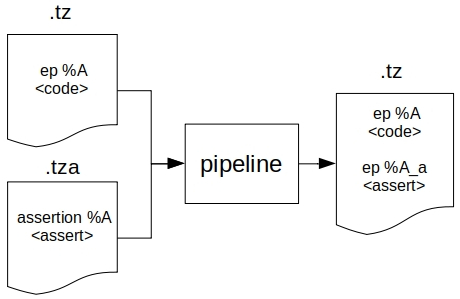
\includegraphics[width=0.5\textwidth]{figures/5-offline_tezos/pipeline_output_mono_ep_basic.jpg}
	\caption{Monolithic assembly - appending assertions as separate entrypoints}
	\label{fig:mono_eps}
\end{figure}

The interface of the contract should make apparent, which of the entrypoints contain production, and which contain their respective assertion code. This can be solved by using fixed tag patterns for assertion entrypoints, which can be derived from the parent entrypoint tag. \figref{fig:mono_eps} proposes the tag suffix ``\texttt{\_a}'' for assertion entrypoints. External transactions should only invoke the production entrypoints.

The assembly in \figref{fig:mono_eps}, however, does not yet provide any means to trigger several test runs per validator. Since the required number of test runs $t$ can only be determined at runtime, it cannot be passed to the validators as a parameter to the validation request. Instead, the contract itself should contain a controller to handle the calculation of $t$ and the initiation of $t$ test runs. Similar to the assertion code, such a controller can be appended as another separate entrypoint, as shown in \figref{fig:monolithic_orchestration}. Instead of invoking the assertion entrypoint (\texttt{A\_a}), the validators would then invoke the controller entrypoint (\texttt{A\_c}), which determines $t$ and invokes (\texttt{A\_a}) $t$ times as an internal operation.
\begin{figure}[h]
\centering
  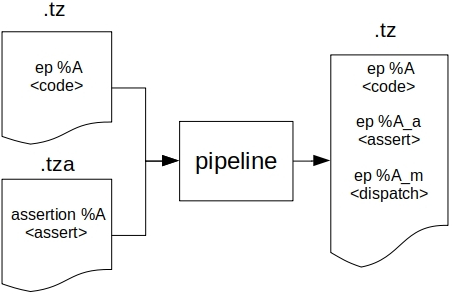
\includegraphics[width=0.5\textwidth]{figures/5-offline_tezos/pipeline_output_mono_ep}
	\caption{Monolithic assembly with separate entrypoints for controller and assertion}
	\label{fig:monolithic_orchestration}
\end{figure}

As a hybrid solution between a monolithic and a modular approach, the controller can be implemented as a separate smart contract, which operates as a proxy. This contract is invoked in place of the monolithic contract, which in turn invokes the original or assertion entrypoints as internal operations. The implementation of the modular part can be adopted from \secref{sec:modular}.

If a developer does not specify an assertion for all entrypoints of the parent contract, invoking their non-existing controller entrypoints would cause a transaction failure. In order to avoid this and increase the robustness, the compiler should generate dummy controllers for empty assertions, which simply return unit (i.e, an empty list of internal operations and the unchanged storage).

\lstref{lst:mono_liq} implements a monolithic contract in Liquidity. The contract contains the two parent entrypoints \texttt{A} (line 3) and \texttt{B} (line 21), and provides an assertion entrypoint \texttt{A\_a} (line 5) for \texttt{A}. Entrypoint \texttt{B} does not have an associated assertion. For both parent entrypoints, it provides the controller entrypoints \texttt{A\_c} (line 7) and \texttt{B\_c} (line 23). Controller \texttt{A\_c} determines the number of test runs in line 8 (the implementation of the formula is omitted here) and creates $t$ internal operations, which invoke the assertion entrypoint with the same parameter (lines 9-17). These are then run in sequence afterwards. Controller \texttt{B\_c}, on the other hand, does not emit any operations and immediately returns. This code can never fail and thus accepts any input value for the parameter.
\lstinputlisting[label=lst:mono_liq, caption=Implementation of a monolithic contract in Liquidity, numbers=left]{listings/monolithic.liq}

\figref{fig:interaction_monolithic} depicts the resulting interactions of the nodes, validators and monolithic smart contracts on the blockchain. The execution model requires a dedicated mode for distributed assertion checking. A possible mechanism to activate this mode is using a special transaction type, which is denoted by \texttt{txa(destination, entrypoint, parameter)} in the graphic. When an operation, such as a transaction or origination, is injected into a node, it is normally propagated to the network after it has been pre-validated by the node. After the injection of \texttt{txa(1, \%A, parameter)}, however, the node broadcasts its derivation \texttt{txa(1, \%A\_c, parameter)} to the network, which invokes the controller entrypoint instead. If this operation finishes successfully for all validators, i.e., no counterexample is published on the network after a certain amount of block cycles, the node can finally broadcast the initial operation as a normal transaction. In case of an assertion failure, the respective validator broadcasts the counterexample including the generated random values. As a consequence of the broadcasted counterexample, the initial operation \texttt{txa(1, \%A, parameter)} should be reverted and rejected by the injecting node. How a counterexample is represented and included on the chain is an unresolved question --- \secref{sec:counterexample} picks this topic up and gives some ideas regarding possible implementations. 

\begin{figure}
\centering
  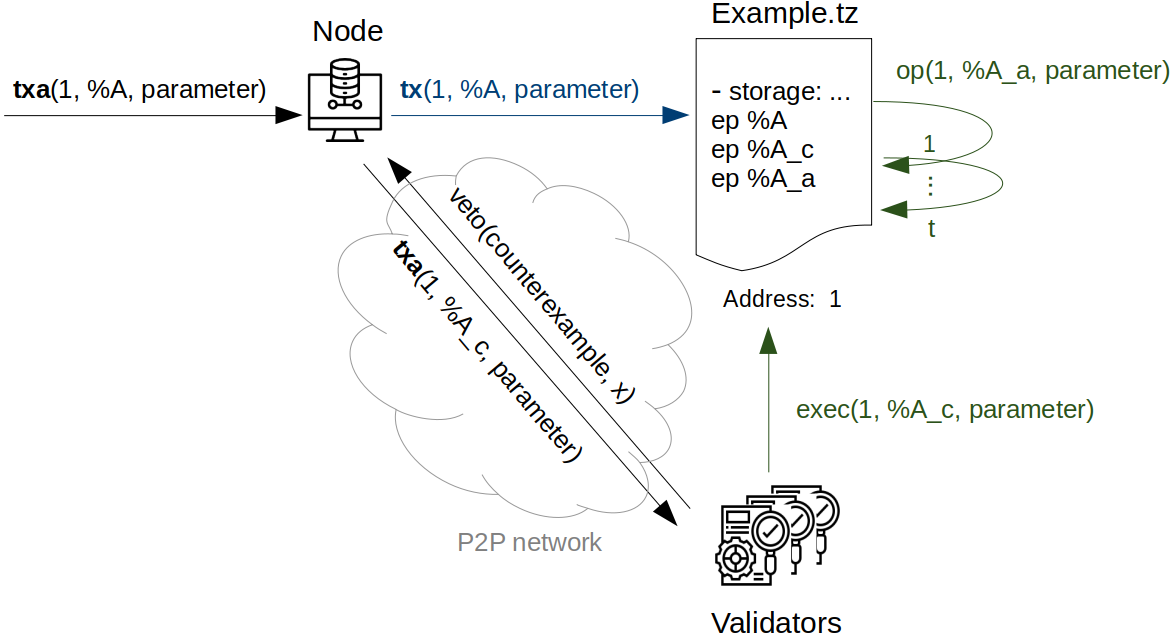
\includegraphics[width=0.9\textwidth]{figures/5-offline_tezos/interaction_monolithic_2}
	\caption{Interaction with a monolithic contract}
	\label{fig:interaction_monolithic}
\end{figure}

This orchestration scheme only works as described when using explicit entrypoint tags for the contract invocations. On the one hand, calling entrypoints implicitly (by wrapping the parameter in the respective sum type constructors) causes a type mismatch for the controller and assertion entrypoints. \lstref{lst:mono} shows the parameter type of the Michelson implementation corresponding to the contract given in \lstref{lst:mono_liq} --- entrypoint \texttt{A} can be invoked implicitly with parameter value \texttt{Left 4}. The respective assertion entrypoint \texttt{A\_a} expects the value as \texttt{Right (Right (Left 4))} and the controller \texttt{A\_c} as \texttt{Right (Right (Right (Left 4)))}. Calling these entrypoints with the same parameter is thus not possible. On the other hand, the explicit tags encode the link between production, controller and assertion code --- omitting them would dissolve all references between them. Hence, implicit entrypoint invocation cannot be supported in the execution mode of assertions. The assertion compiler thus needs to enforce the use of explicit entrypoints in the parameter type declarations and the \texttt{txa} operation type must expect a mandatory entrypoint specification as an argument.
\lstinputlisting[label=lst:mono, language=Michelson, caption=Skeleton of a monolithic contract in Michelson, numbers=left, float]{listings/monolithic.tz}

This thesis does not go into more detail about how the described execution model for a monolithic orchestration is designed and implemented in the blockchain protocol. What needs to be considered in future work concerning the protocol design is the separate execution mode, a dedicated operation type as proposed above, the derivation of a transaction which attempts to find a counterexample, the handling of assertion failures and the exclusive acceptance of the off-chain computation (and thus the transaction submitting it) or the counterexample.

\subsubsection{Evaluation of the Monolithic Approach}
The purely and hybrid monolithic implementation each have strengths and weaknesses. Generally, they share a pivotal disadvantage - they require a modification of the parent contract. This complicates the compilation process substantially and precludes the integration of assertions to contracts which have already been deployed to the blockchain. \lstref{lst:mono} shows how the parameter type and branching within the code body have to be adapted compared to the original parent contract in \lstref{lst:mono_parent}. Since the monolithic assembly results in deeper parameter and code nestings, the overall complexity of the contract increases and may obscure the production code.
\lstinputlisting[label=lst:mono_parent, language=Michelson, caption=Skeleton of the pure parent contract in Michelson, numbers=left]{listings/monolithic_parent.tz}

Another shortcoming is the missing support of implicit entrypoint invocations. Even though the previously mentioned measures can prevent transactions failures, this still poses a restriction in the interaction with smart contracts. 

Due to the tight coupling of parent and assertion code, this approach is also inflexible. Adaptions to either the assertion or the parent contract require a complete recompilation and origination of the monolithic contract. The hybrid solution resolves some of the tight coupling, as a new version of the controller contract can be originated independently of the monolithic contract.

Besides these disadvantages, the monolithic approach provides a distinct advantage: the production and controller entrypoints can be invoked independently, implicating that the validators do not have to run the production code while checking the assertion. Conversely, the assertion code is not rerun if the parameter was validated and the actual transaction is broadcast to the network. This reduces the transaction cost for the user, as well as the overall computational footprint of the transaction and the validation in the network.

\subsection{Modular Orchestration}\label{sec:modular}
In the modular approach, the controller and each of the assertions are originated as separate contracts on the blockchain. The controller mirrors the interface of the parent contract, while each assertion contract only features a single entrypoint, which corresponds to the raw type of the associated parent entrypoint. By keeping the assertion code separated, the parent contract remains pure and does not have to be modified. Similar to the hybrid solution mentioned in the monolithic approach, the controller calls the respective assertion contract $t$ times as an internal operation, before invoking the parent contract as operation $t+1$. In the case of empty assertions, the controller acts as a direct gateway by invoking the parent contract immediately. Corresponding to this architecture, the toolchain returns $m + 1$ contracts, where $m$ is the number of specified assertions in the input. The code assembly and output of the toolchain is outlined in \figref{fig:modular_assembly}.
\begin{figure}[h]
\centering
  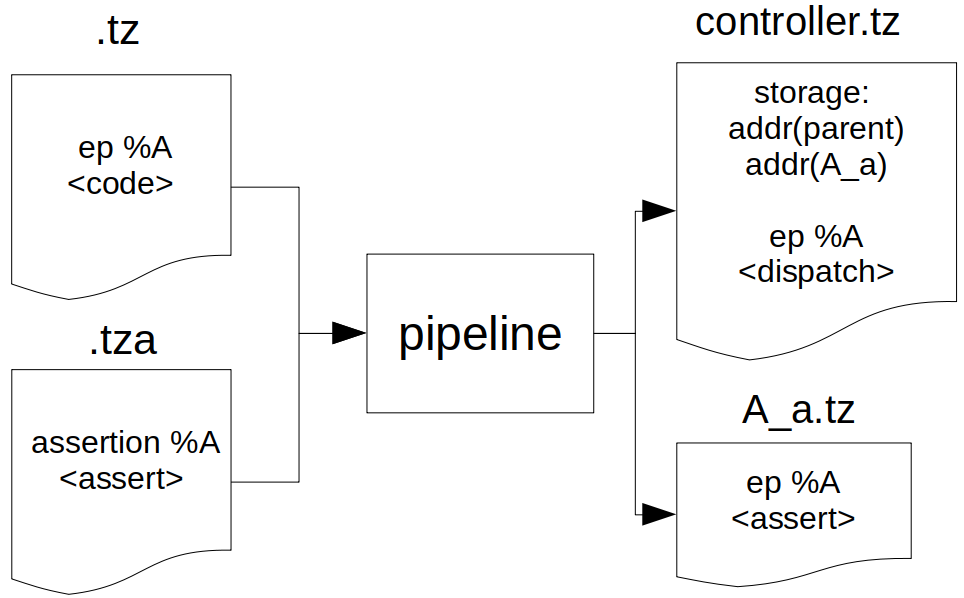
\includegraphics[width=0.6\textwidth]{figures/5-offline_tezos/pipeline_output_modular.png}
	\caption{Modular assembly of assertion and manager code}
	\label{fig:modular_assembly}
\end{figure}

In order to link the separate contracts to each other, the controller needs to have a reference to the other contract modules. This results in a fixed origination order --- the assertion and parent contracts must be originated first, and their addresses are passed to the controller as initial storage values. A proposed structure of the storage is a map from a unique identifier to an address. The entrypoints of the controller can then look up the addresses of the parent and the respective assertion contract with an assigned identifier. The assignment of the identifiers is hard-wired during the compilation, as is demonstrated in the rudimentary and simplified Liquidity implementation of a controller contract in \lstref{lst:manager_modular}. The corresponding storage initiation for this contract is the map $\lbrace 0 \rightarrow \langle \text{address parent} \rangle; 1 \rightarrow \langle \text{address assertion} \rangle \rbrace$ . The hard-wired identifiers are used in lines 5 and 6 to retrieve the addresses from the storage.
\lstinputlisting[label=lst:manager_modular, caption=Implementation of the modular controller in simplified Liquidity, language=Michelson, numbers=left]{listings/controller_basic.liq}

The interaction with the modular contracts is shown in \figref{fig:interaction_modular}. Even though the transactions shown in the diagram state an explicit entrypoint tag, the scheme also supports implicit entrypoint invocations. Invocations of the assertion contract pass the parameter as a raw value. The general execution model is similar to the model for the monolithic approach, but requires a few modifications; because the controller mirrors the interface of the parent contract, the \texttt{txa} operation can be broadcast to the network directly --- a derivation to a distinct transaction, which calls the assertion selectively, is not necessary. If none of the validators publish a counterexample, the initial transaction is broadcasted to the network as a normal operation to be included in a block. This transaction will inevitably rerun the assertion code in the normal execution mode (as it invokes the controller). Hence, the \texttt{random} instruction should not cause an internal operation to fail in the normal execution mode of the VM. This could be solved by marking these internal operations with the operation result ``Skipped'' (cf. \secref{sec:internal_ops}), or by introducing a dedicated result type for this case. 
\begin{figure}[h]
\centering
  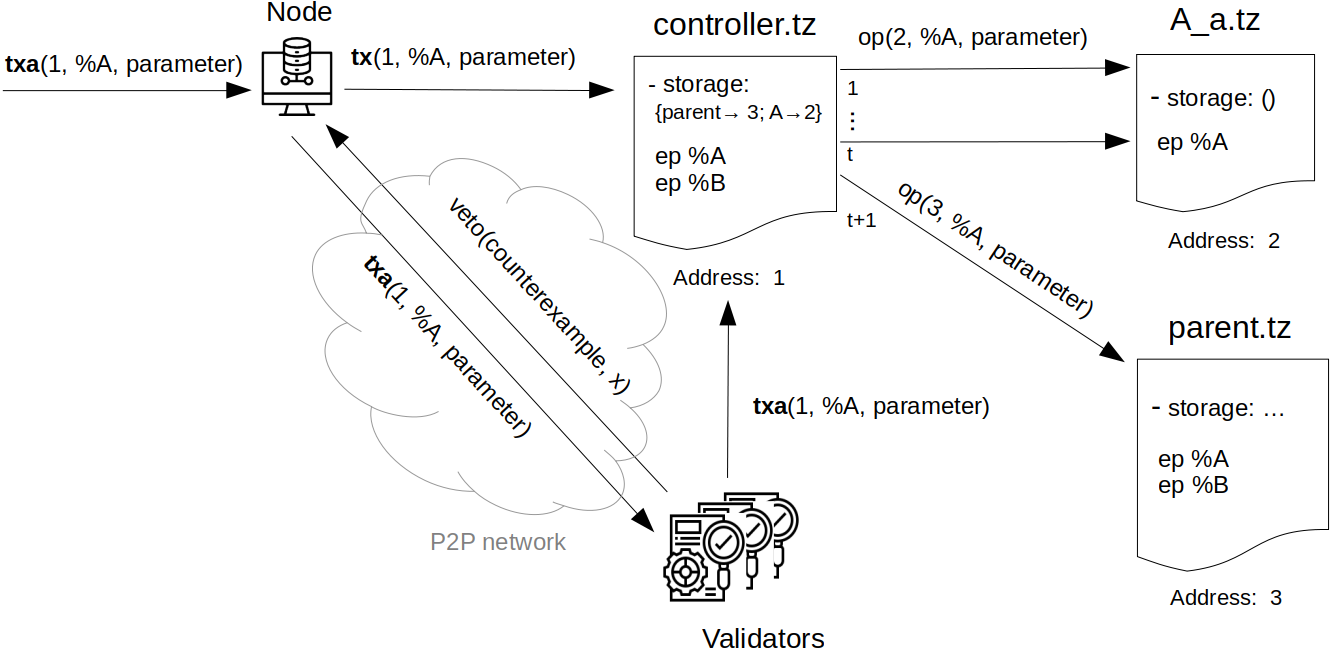
\includegraphics[width=\textwidth]{figures/5-offline_tezos/interaction_modular.png}
	\caption{Interaction with modular contracts}
	\label{fig:interaction_modular}
\end{figure}

\subsubsection{Evaluation of the Modular Approach}
This approach resolves the two crucial problems of the monolithic orchestration: by mirroring the interface of the parent contract, the parameters passed to the manager contract can be forwarded directly to the parent contract, regardless of whether the default or an explicit entrypoint was called. Furthermore, the parent contract does not need to be modified, which leads to a much simpler compilation process and allows to extend already originated contracts with assertions. Due to its modularity, adaptions to either contract do not necessarily require a recompilation and origination of all components, as the controller is the only component with tight coupling. In order to reduce this coupling, one could be inclined to add a setter entrypoint to the controller (as a sort of dependency injection). This, however, would break the mirroring of the parent contract and is thus not possible without annulling one of the key strengths of the design.

The approach essentially exhibits two weaknesses: firstly, the assertion and the parent cannot be called separately. As a result, the production code is run by every validator while searching for counterexamples. Moreover, the assertion code is also run when validating a block containing the accepted transaction. This increases the transaction cost for the user and requires a higher computational effort by the whole network. Secondly, it exposes a security vulnerability, given that assertions can be bypassed by calling the parent contract directly. This iteration of the design does not demand to close this vulnerability, hence possible solutions are not discussed in this thesis.

Even though the monolithic approach is expected to be more efficient, the toolchain implementation described in the following sections is based on the modular architecture. It is simple to implement, requires less modifications to the blockchain protocol and provides more flexibility.

\section{Backend Implementation}\label{sec:backend_impl}
The following sections describe the tasks and implementation of the pipeline stages in the toolchain backend.
\begin{figure}[h]
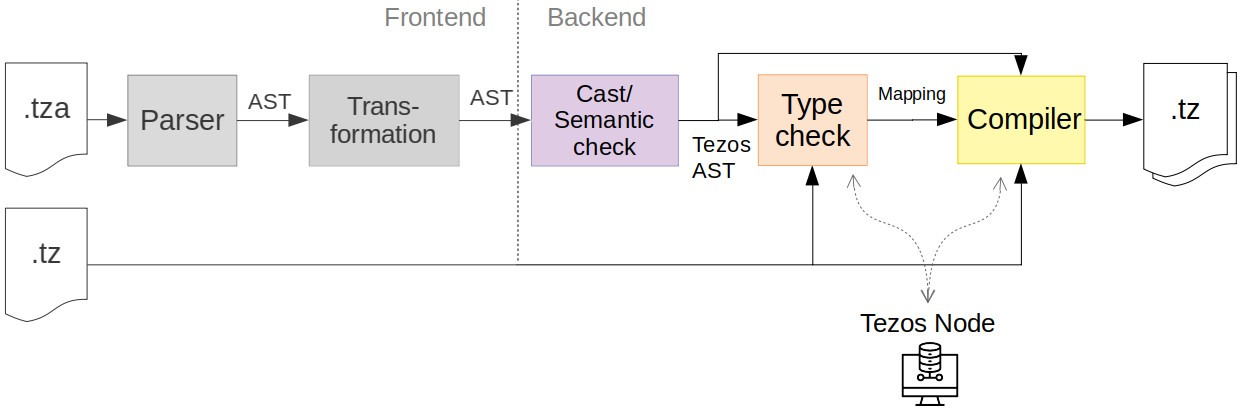
\includegraphics[width=\linewidth]{figures/5-offline_tezos/pipeline_backend}
\caption{The stages of Tezos-specific backend of the compilation pipeline}
\label{fig:pipeline_backend}
\end{figure}

\subsection{Interaction with Tezos Nodes}
Some stages of the backend have to interact with a Tezos node, e.g. to retrieve information from the blockchain. For this, the backend uses the Tezos client libraries, which provide high-level functions wrapping RPCs to a configured node. The command-line interface of the toolchain provides options for configuring the host address and port of the RPC interface to connect to a specific local or public node. By default, the toolchain tries to connect to a local node on the default port.

\subsection{Semantic Analysis}
After the transformation, the frontend passes a list of ASTs to the backend. Because the frontend was designed to be generic, they may contain type, operations or expressions which are not supported by the target language. Therefore, the semantic check should reject any input which cannot be translated to Michelson.

As an additional restriction, quantifiers should only bind variables of primitive data types. As the majority of use-cases seem to require quantification over numerical values, the current implementation of the semantic check restricts predicate variables to the types \texttt{int} and \texttt{nat}. Future iterations of the toolchain and protocol may add support for other primitive types, such as \texttt{string} or \texttt{bytes}.

Semantic rules imposed by Michelson do not have to be checked explicitly by the toolchain --- the RPC interface of Tezos nodes provides a function to parse and type check Michelson programs, which can be used to verify the correctness of the compilation result and reject any assertions containing type or other semantic errors.

If the semantic check was successful, the module returns the assertions as a list of Tezos-specific ASTs. \lstref{lst:tezos_ast_type} shows the toplevel definition of this AST type.
\begin{lstlisting}[label=lst:tezos_ast_type, language=, numbers=none, caption=Toplevel Tezos-specific AST type definition in OCaml]
type tezos_ast =
  {entrypoint : string * pattern; body : assertion}
\end{lstlisting}
As Tezos is currently the only supported target platform, the type differs only slightly from the generic type. If the assertion does not specify an explicit entrypoint tag, the optional value is replaced with Tezos' notation for the default entrypoint. The subtree types for the parameter pattern and the assertion remain equivalent to the generic subtree types.

\subsection{Type Check}\label{sec:typecheck}
Given a list of Tezos-specific ASTs, the task of the type checker is to link each AST to the respective entrypoint of the parent contract. This stage module can therefore also be referred to as the ''linker``. The linking is needed by the compiler to correctly assemble and type the controller and assertion contracts. As a simple example, the linker should correctly assign the AST of the first assertion in \texttt{Example.tza} (\lstref{lst:linker_assertion}) to entrypoint A and the second assertion to entrypoint B of the parent contract \texttt{Example.tz} (\lstref{lst:linker_parent}). 

\vspace{\baselineskip}
\noindent
\begin{minipage}{.45\textwidth}
\begin{lstlisting}[label=lst:linker_parent, numbers=none, language=Michelson, caption=Example.tz]
parameter (or (int %A)
              (string %B));
...
\end{lstlisting}
\end{minipage}\hfill
\begin{minipage}{.5\textwidth}
\begin{lstlisting}[label=lst:linker_assertion, numbers=none, language=Assertion, caption=Example.tza]
(entrypoint %A (i : int) ...)
(entrypoint %B (s : string) ...)
\end{lstlisting}
\end{minipage}
\vspace{\baselineskip}

Because explicit entrypoint tags are optional in Michelson contracts, the linking is primarily done by type matching between the declared parameter types in the parent and parameter patterns in the assertions. If the type matching does not result in an unambiguous assignment between an assertion and an entrypoint, i.e., the parameter pattern matches the type of several entrypoints, the linker considers the specified tags in an effort to resolve the ambiguity. The linking fails if no injective, non-surjective mapping from the set of assertions to the set of entrypoints was found regardless. 

\subsubsection{Parameter Patterns Revisited}
As explained in \secref{sec:tezos}, transactions on Tezos can invoke entrypoints implicitly by invoking the default entrypoint and wrapping the parameter value into the respective union type constructors. Alternatively, they can be called explicitly by stating an entrypoint tag and passing the raw parameter value as an argument. The same principle applies for the specification of assertions - when omitting the tag in the assertion signature, the parameter pattern must be declared in respect to the default entrypoint. If the assertion states an explicit tag, it may declare a pattern of the raw parameter type. \lstref{lst:impl_expl} shows two valid assertion specifications for entrypoint A of the contract \texttt{Example.tz} (\lstref{lst:linker_parent}) --- the first specification uses an explicit tag paired with the pattern of the raw parameter type, while the second does not specify a tag and declares the parameter pattern with respect to the default entrypoint, i.e, wrapped into the sum type constructor \texttt{left}. 
\begin{lstlisting}[language=Assertion, numbers=none, caption=Explicit and implicit parameter specification in assertions, label=lst:impl_expl]
(entrypoint %A (i : int) ...)
(entrypoint (left (i : int)) ...)
\end{lstlisting}

The tags given in the assertion specification do not necessarily have to be identical with the tags of the parent contract; they may be chosen differently for documentation purposes, particularly if the parent contract does not state any tags. However, tags can and should be used to resolve ambiguity in the linking between assertions and entrypoints by mirroring the entrypoint tags of the parent contract.

\subsubsection{Resolving ambiguity}
\lstref{lst:ambiguity_assertion} provides four examples of assertions which cannot be linked unambiguously to an entrypoint of the contract given in \lstref{lst:ambiguity_parent}. Since the entrypoints of \texttt{Example2.tz} have the same raw parameter type \texttt{int}, and none of the given assertions tags refer to one of them explicitly, the linker cannot infer which entrypoint they refer to. In all four cases, providing an explicit tag (\texttt{A} or \texttt{B}) can resolve the ambiguity. If the parent entrypoint does not specify a tag, the ambiguity can be resolved by omitting the tag and specifying the parameter pattern in respect to the default entrypoint, e.g. \texttt{left \_} or \texttt{right (i : int)}. 

\vspace{\baselineskip}
\noindent
\begin{minipage}{.4\textwidth}
\begin{lstlisting}[label=lst:ambiguity_parent, numbers=none, language=Michelson, caption=Example2.tz]
parameter (or (int %A)
              (int %B));
...
\end{lstlisting}
\end{minipage}\hfill
\begin{minipage}{.5\textwidth}
\begin{lstlisting}[label=lst:ambiguity_assertion, language=Assertion, caption=Ambiguous assertions for Example2.tz]
(entrypoint _ ...)
(entrypoint %C _ ...)
(entrypoint %D i ...)
(entrypoint %E (i : int)
\end{lstlisting}
\end{minipage}
\vspace{\baselineskip}

Another type of ambiguity is caused by the fact that entrypoints can be sub-entrypoints of others. As an example, consider the parameter type of contract \texttt{Example3} in \lstref{lst:overlap_parent}. Entrypoints \texttt{B} and \texttt{C} are sub-entrypoints of \texttt{BC} --- invoking \texttt{BC} will inevitably result in an invocation of either \texttt{B} or \texttt{C}, depending on the parameter value. Thus, assertions may ``overlap'' if a separate assertion is declared for a super- and a sub-entrypoint and result in two assertion specifications for the same entrypoint, as is demonstrated in \lstref{lst:overlap_assertion}. The linker detects such overlapping assertions and rejects assertion specifications containing such. Hence, a valid assertion contract can specify an assertion for entrypoint \texttt{AB} only, or for entrypoints \texttt{A} and \texttt{B}, but not for \texttt{AB}. 

\vspace{\baselineskip}
\noindent
\begin{minipage}{.45\textwidth}
\begin{lstlisting}[label=lst:overlap_parent, numbers=none, language=Michelson, caption=Example3.tz]
parameter (or %AB (int %A)
                  (int %B));
...
\end{lstlisting}
\end{minipage}\hfill
\begin{minipage}{.5\textwidth}
\begin{lstlisting}[label=lst:overlap_assertion, numbers=none, language=Assertion, caption=Example3.tza with overlapping assertions]
(entrypoint %AB (left  i) ...)
(entrypoint %A j ...)
\end{lstlisting}
\end{minipage}
\vspace{\baselineskip}

\subsubsection{Linking Process}
As a first step, the linker retrieves and parses the parameter type of the parent contract. The parent contract is provided by the user as a file, a blockchain address, or a raw string. In case the contract is given as an address, the code is retrieved from the blockchain. From the parsed parameter type, a list of all named and anonymous entrypoints with their raw input types is extracted. For these steps, the Tezos client and protocol libraries are utilized. 

Based on the extracted pool of entrypoints and the list of assertion ASTs, the linker then iteratively builds a mapping between entrypoints and assertions. The parameter pattern of each assertion AST is compared to the parameter type of all entrypoints in the pool. All matching entrypoints are collected in a list. If this list is empty, linking the assertion fails due to a type mismatch and the pipeline terminates. In case the list contains several entrypoints, the linker considers the tags in order to resolve the ambiguity. If the tags do not lead to a resolution, the pipeline terminates due to an ambiguous assertion specification. Lists containing exactly one match can be resolved to an assignment directly. After an AST could be linked to an entrypoint, the assignment is added to the mapping and the matching entrypoint is removed from the pool of unlinked entrypoints. Additionally, all sub- and super-entrypoints are removed from the pool. By removing these entrypoints, the linker is able to detect duplicate or overlapping assertions.

After successfully finding a valid assignment for all assertions, the linker returns the mapping. Because entrypoints can be anonymous, the mapping represents the entrypoints with the constructor nesting of their parameters. \lstref{lst:unionpath} shows the definition of the type for such a representation.
\begin{lstlisting}[label=lst:unionpath, language=, numbers=none, caption=Type representing entrypoints according to the union constructor nesting]
type union_path = Left of union_path
                | Right of union_path
                | T
\end{lstlisting}
Using this type, entrypoints \texttt{A} and \texttt{B} of \texttt{Example.tz}, for instance, are represented by \texttt{Left T} and \texttt{Right T}, while the default entrypoint is represented by \texttt{T}. Given \texttt{Example.tza}, the linker thus returns the mapping \\
\texttt{\{ Left T \textrightarrow \, <AST assertion A>; Right T \textrightarrow \, <AST assertion B>\} }.

\subsection{Compiler}\label{sec:compiler}
The compiler finally translates the transformed and type checked assertion ASTs to Michelson contracts according to the modular orchestration scheme. Assertion and parent contract are thus assembled as depicted in \figref{fig:modular_assembly}. The compilation stage was not implemented within the scope of this thesis, but the following subsections describe the compilation procedures for generating the assertion and controller contracts. Furthermore, this section discusses the alternative of compiling to a high-level language as an intermediate representation, instead of compiling to Michelson directly.

With Michelson as the compilation target language, the compiler has to generate code for a stack machine. After compilation, the Michelson programs can be validated for correctness by the Tezos node, which will intercept any assertions containing type errors. After this sanity-check, the compiler outputs the target code for the controller and assertion contracts. As an additional output, it should return a piece of template code for the correct storage initialization of the controller contract. Before originating the controller contract, the user fills in the blockchain addresses of the other modules.

\subsubsection{Compilation of the Assertion Contracts}
The assertion ASTs are independent and can thus be compiled in isolation to separate Michelson contracts. Because they only have a single entrypoint, the parameter type corresponds to the raw parameter type of the parent entrypoint. If the parameter pattern in the assertion does not contain any wildcards, the parameter type can be derived directly from the pattern. Otherwise, the compiler has to infer the type from the parent contract.

If the pattern excludes any special values of the data type (e.g., \texttt{cons head tail} excludes empty lists), the generated code should reflect this. It has not been specified yet, if excluded values should never or always cause the assertion to fail. In the example of \texttt{cons} and assuming excluded values pass the assertion, the generated code could contain the branching shown in \lstref{lst:cons}. The branch in line 1 is executed if the list contains at least one element, and should contain the assertion code. If the list is empty, the branch in line 2 should simply return successfully. 
\begin{lstlisting}[language=Michelson, label=lst:cons, caption=Exclusion of empty lists in the assertion]
IF_CONS ( <assertion body> )
        ( <return ([], ())>)
\end{lstlisting}

To simplify the compilation, the generated code of the assertion body and the parameter type can be plugged into a template containing the necessary boilerplate code for a contract. Such a template is shown in \lstref{lst:contract_templ} --- the placeholders \texttt{<?>} mark the locations where the individual code is inserted. Since assertions do not use any storage as of now, the storage type is set to unit. Lines 3-5 prepare the stack, s.t. the parameter and storage are the two top elements. The lines below the placeholder for the body leave the stack according to calling convention, i.e., the program returns an empty list of internal operations and the unit storage.
\lstinputlisting[label=lst:contract_templ, language=Michelson, caption=Template code for assertion contracts in Michelson, numbers=left]{listings/assertion_template.tz}

\subsubsection{Compilation of the Controller Contract}
The generation of the \texttt{parameter} and \texttt{storage} primitives for the controller contract is trivial. Given that the controller acts as a proxy, the parameter type can be copied from the parent contract. Assuming that the proposal for the storage type from \lstref{lst:manager_modular} is adopted, the storage type is always the same, i.e., \texttt{(map int address)}. The code body is generated recursively based on the parameter type. It consists of two types of entrypoints, which either act as a direct gateway to the parent contract in the case of empty assertions, or trigger an assertion check before invoking the parent.

\paragraph{Gateway entrypoints}
The code of gateway entrypoints only has to execute two steps; first, the address of the parent contract is read from the storage. It then creates an internal operation to this address, passing along the original parameter and funds. Assuming the parent address is always stored under the same key, e.g. with id 0, such gateways can be generated as fixed boilerplate code.

\paragraph{Assertion entrypoints}
If the entrypoint should trigger an assertion, the compiler has to generate code executing the following steps:
\begin{enumerate}
\itemsep-0.5em
\item Read the addresses from the assertion and parent contract from storage
\item Calculate the number of test runs $t$
\item Compile a list of $t$ internal operations invoking the assertion with the raw parameter
\item Create an internal operation calling the parent contract, passing the original parameter and funds
\item Return (i.e., push to the stack) a list of all internal operations and the unchanged storage
\end{enumerate}
\secref{sec:prob_threshold} stated a formula to determine the total number $t_{total}$ of required test runs, given a probability threshold $c$ and the size of the search space $n$. From $t_{total}$ the number of test runs $t$ per validator can be calculated according to \eqref{eq:t_validator}. Since $n$ can only be obtained at runtime, the compiler needs to derive a formula to determine this value from the ranges of the random generators. \secref{sec:sample_space} already gave some examples of this. 
The threshold $c$, on the other hand, must be given as a parameter to the compiler. Therefore, the command line interface of the toolchain should provide an option to set this threshold.

\paragraph{Algorithm}
Algorithm \ref{alg:compile_manager} shows the outline of a simplified algorithm which builds the code body of the controller. It recursively iterates over the parameter type and builds the body by nesting \texttt{IF\_LEFT} instructions (cf. \lstref{lst:entrypoints}). Within the entrypoint branches, the compiler either generates gateway or assertion triggering code (based on the mapping given by the linker).

\begin{algorithm}
\caption{Simplified recursive algorithm for building the controller}\label{alg:compile_manager}
	\begin{algorithmic}[1]
	\State global storage = \{0: <parent>\}
	\State global i = 1
	\Function{compileController}{parameter type}
	\If{ty = Or(l,r)}
	\State codeLeft = "IF\_LEFT {" + compile(l) + "}"
	\State codeRight = "{" + compile(r) + "}"
	\State \Return codeLeft + codeRight
	\Else
	\If{entrypoint has assertion}
	\State code = generateAssertionTrigger(parameter type, i, assertion)
	\State storage.add(i++, entrypoint tag)
	\Else
	\State code = generateGateway()
	\EndIf
	\State \Return code
	\EndIf
	\EndFunction
	\end{algorithmic}
\end{algorithm}

During this recursion, the compiler also builds the address map for the storage, such that the entrypoints can look up the addresses of the assertion and parent contracts during runtime. To this end, it keeps the counter \texttt{i} to create unique IDs for each entrypoint with an assertion --- this ID is then hard-wired into the instruction accessing the storage within this entrypoint. The address of the parent contract is always stored under ID 0. 

After compilation, this map is translated to a template for a Michelson value of type \texttt{map} and returned to the user. Because the addresses are not known at compilation time, the map values should be descriptive place-holders, s.t. the user can replace them with the corresponding addresses after the respective contracts have been originated. After the user replaced the placeholders with the actual addresses, this Michelson value should then be passed to the origination as the initial storage value. As an example, the compilation of the controller contract for \texttt{Example.tz} and \texttt{Example.tza} in Listings \ref{lst:linker_parent} and \ref{lst:linker_assertion} could return the following template:\\ \texttt{(Elt 0 <addr parent>; Elt 1 <addr A\_a>; Elt 2 <addr B\_a>)}.

In order to provide a detailed example, appendix \ref{apx:controller_michelson} contains the full Michelson code of a controller contract with one gateway and one assertion entrypoint. The code was generated by the Liquidity compiler from the source given in appendix \ref{apx:controller_liq}, which provides a more compact and readable representation of the program logic.

\subsubsection{Compiling to an Intermediate Representation}\label{sec:IR}
Instead of generating Michelson code directly, the compiler could also generate code in one of the high-level languages listed in \secref{sec:languages}. They all provide compilers targeting Michelson, and can thus serve as an intermediate representation (IR) of the contract code.

It depends on the language how the compiler of the IR can be integrated into the toolchain. The Ligo project builds their compiler into a \texttt{dune}\footnote{dune \cite{dune} is a build system for OCaml} library, which can be imported directly into the code base of the toolchain. This keeps the pipeline coherent and would allow to output Michelson contracts without any intermediate steps. If the compiler cannot be embedded directly into the toolchain (as is the case with Liquidity), the output of the toolchain would have to be compiled manually to Michelson in a separate step, as depicted in \figref{fig:pipeline_liq}.

\begin{figure}[h]
\centering
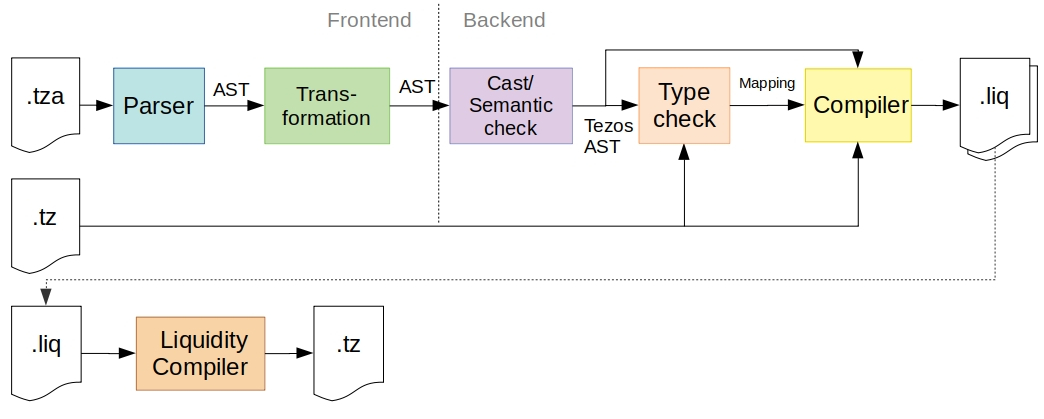
\includegraphics[width=\linewidth]{figures/5-offline_tezos/pipeline_liq}
\caption{Pipeline with IR compilation and an external compiler}
\label{fig:pipeline_liq}
\end{figure}

\paragraph{Comparison to direct compilation}
This approach takes advantage of the usually more sophisticated high-level language compilers; they may provide options for optimizing generated code and are already thoroughly tested. In contrast to large and obscure Michelson programs, the output is more comprehensible and thus easier to test and verify.

The crucial disadvantage of the IR approach is the introduction of an external dependency. The compiler of the respective language has to be extended with the \texttt{random} instruction as well, which requires forking the project. Furthermore, one has to rely on continuous support of new protocol versions in the root project, and integrate the updates into the own code base regularly.

However, a realistic use-case for using Liquidity as an IR is the implementation of the monolithic orchestration scheme. In Liquidity, each entrypoint is declared as a function expecting a parameter and the current storage. During compilation, the contract parameter type and code branching is composed according to the order of functions given in the source file. For instance, the entrypoint declarations in \lstref{lst:liq_eps} are compiled to the contract parameter type \texttt{(or (int \%A) (int \%B))} and two branches in the code body.  
\begin{lstlisting}[numbers=none, label=lst:liq_eps, caption=Entrypoint declarations in Liquidity]
let%entry A (a : int) storage = ...
let%entry B (b : int) storage = ...
\end{lstlisting}
As the Liquidity project provides a decompiler to translate Michelson contracts into Liquidity programs, the compiled assertion functions can simply be appended to the decompiled parent contract. This results in an assembly scheme as depicted in \figref{fig:liq_assembly} and outsources most of the compilation complexity to the Liquidity compiler.

\begin{figure}[t]
\centering
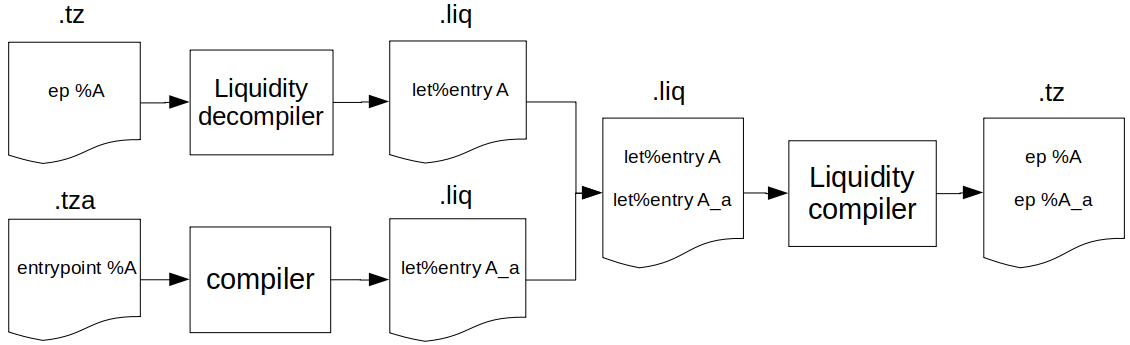
\includegraphics[width=\linewidth]{figures/5-offline_tezos/liquidity_assembly}
\caption{Monolithic assembly using Liquidity as IR}
\label{fig:liq_assembly}
\end{figure}

\section{Cost Analysis and Evaluation}\label{sec:cost_analysis_distributed}
In this section, the costs of checking a formula, with the proposed approach and implementation for distributed assertion checking, are evaluated. \secref{sec:usecase_cost} already determined the cost for a local validation as a benchmark. It stated \eqref{eq:gas_transaction} to calculate the gas consumption of a transaction including internal operations. It identified the gas consumption of deserialization, data parsing and interpretation as growing factors, as they depend on the size of the input parameter.

According to the orchestration scheme, each validator executes $t+2$ operations with the same input parameter $p$. Since they apply lazily, the deserialization cost for the parameter and assertion code only have to be paid once. In addition to the interpretation cost, the reading, parsing and base costs have to be paid for each internal operation. 
\begin{align}\label{eq:gas_validator}
\begin{split}
GasConsumed_{validator}(p) > \quad t * (&base\, gas \\
&+ gasParsing(p) \\
&+ gasRead(C_{assertion}) \\
&+ gasParsing(C_{assertion}) \\
&+ gasInterpretation(C_{assertion})) \\
\end{split}
\end{align}
Based on the resulting inequality in \eqref{eq:gas_validator}, which specifies the costs incurred by each internal operation invoking the assertion contract as a basis of the total gas consumption per validator, it must be concluded that the overall gas consumption of the distributed validation is higher than in the case of a local validation.

The distributed approach was benchmarked by implementing the orchestration scheme for the two minimal dummy contracts \texttt{Foo} and \texttt{Bar} given in \secref{sec:usecase_cost}. Appendix \ref{apx:foobar_distributed} contains the Michelson code for the controller, assertion and parent contracts. In order to preserve comparability between the benchmark of the local and the distributed implementation, the controller contracts were configured with a probability threshold $c = \frac{1}{e}$, s.t. that the necessary number of test runs is equal to the sizes of the search spaces. \figref{fig:cost_distributed} shows the reported gas consumption per validator for different input sizes on the test network Delphinet. Since the effective number of test runs is always a multiple of 32, the cost functions approximate a step function.  

\begin{figure}[t]
\centering
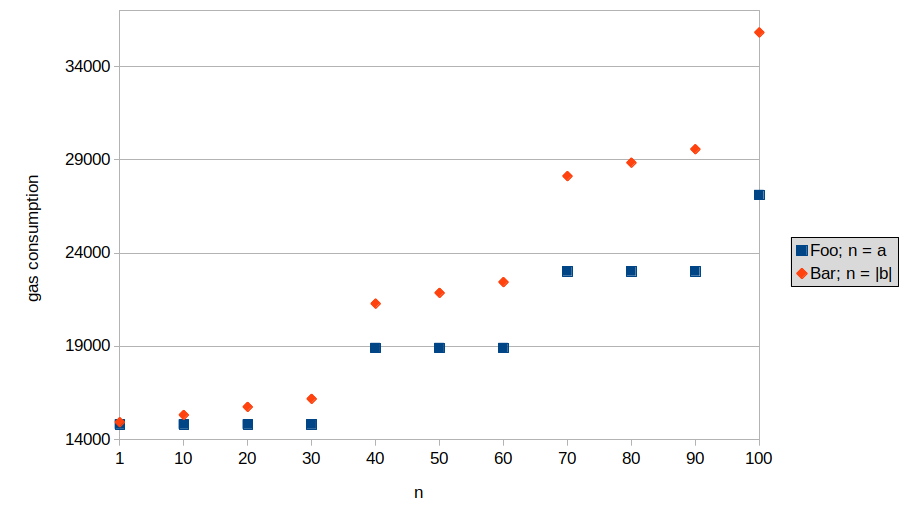
\includegraphics[width=\linewidth]{figures/5-offline_tezos/cost_analysis}
\caption{Gas consumption per validator for different input sizes n}
\label{fig:cost_distributed}
\end{figure}

The results show, that the cost incurred by a single validator, checking a subset of a search space of size $n$, is already considerably higher than a complete validation in a local approach (cf. \figref{sec:usecase_cost}). In the case of the list parameter (contract \texttt{Bar}), the gas consumption even increases exponentially due to the multiplied reading and parsing costs. Moreover, the cost-performance ratio is also worse, as the probability of accepting an invalid parameter with the given configuration is 37\% in the worst case.

In conclusion to these results, the proposed implementation of the distributed scheme has to be evaluated as inefficient and unable to achieve an improvement regarding the scalability of applications on Tezos. However, by reducing the required computation per node to a fraction of the verification, it has the potential to reduce the computational footprint of the transaction within the network. As a prerequisite, it is crucial to lower the costs of the verification. This thesis already mentioned some alternative approaches and implementations, which might achieve this; \secref{sec:alt_random} introduces the possibility to coordinate the validators in a systematic iteration of the search space. Although this does not reduce the cost per test run, it reduces the quantity of necessary test runs to achieve a reliable result. Furthermore, this chapter described several other orchestration schemes, some of which reduce the number of emitted internal operations. As the inter-contract communication accounts for most of the gas consumption in the modular approach, avoiding them is an effective way of reducing the costs. In this regard, a concrete improvement of the proposed architecture could be to merge the controller and assertion code into a single contract. This corresponds, to some extend, to the inverse hybrid architecture as described in \secref{sec:monolithic}. Instead of $t+1$ internal operations, this only requires a single internal operation calling the parent contract (provided that the controller an assertion code are merged into one entrypoint).

\section{Open Questions}
Two remaining aspects of the off-chain design could not be addressed in detail by this thesis. These aspects are outlined briefly in the following sections.

\subsection{Representing Counterexamples}\label{sec:counterexample}
It remains to be specified, how counterexamples are represented within the network. The interaction scheme in \figref{fig:interaction_modular} suggests, that validators publish a counterexample to the network in case of a failed assertion. For this, the validators have to obtain the randomly generated values from within the execution context of the VM. With the \texttt{failwith} instruction, the top element of the stack is exposed, allowing to return an interpretable expression from the execution context. The generated values can thus be returned as a single value, a (nested) pair or a list. To allow other validators to check the assertion with a specific set of values, a modified version of the assertion code must be available on the blockchain. Instead of generating random values, this version should take these values as input parameters. Hence, the validator could create a normal transaction invoking this code with the values returned by the \texttt{failwith} instruction and publish it to the network. The counterexample is then validated like any other transaction on the blockchain. Nodes publishing false counterexamples should be penalized in order to prevent denial of service attacks. After a counterexample has been validated, the respective transaction submitting the invalid off-chain computation should be rejected. Consequently, the transaction and counterexample need to be relatable, e.g. by using an operation hash as an ID. 

To implement this scheme, the compiler has to generate one more contract per assertion. In addition, the assertion contract needs to know about the address of the counterexample contract, and return the address together with the generated values in case of a failure. This requires an adjustment of the storage type of the assertion contract and changes the order of origination to:
\begin{enumerate}
\itemsep-0.5em
\item \texttt{Origination(parent)}, \texttt{Origination(counterexample)}
\item \texttt{Origination(assertion, address counterexample)}
\item \texttt{Origination(controller, [address assertion], address parent)} 
\end{enumerate}

\subsection{Multi-slot Validators}
The proposed implementation assumes that all 32 validators of the current block cycle execute a determined number of test runs. In fact, as mentioned in the section describing Tezos' proof-of-stake mechanism, a validator may have been assigned several endorsement slots per cycle. Since these validators only execute the assertion once, the test runs for the other endorsement slots are neglected. As a result, the error rate of the assertion check is not deterministic and may exceed the configured threshold. This issue should be addressed by the protocol design --- multi-slot validators should execute the assertion check for each of their endorsement slots.
    \chapter{Conclusion and outlook}\label{chap:conclusion}
In order to make use of off-chain computations in smart contracts, this thesis proposed an approach that engages the validators of the blockchain network in a distributed effort to check assertions over input parameters. It covered the partially generic off-chain component of the design and implementation of this approach, while also providing some projections and considerations for the Tezos specific protocol design.

As a first step, it identified properties that can be checked with the proposed scheme, represented by a set of formulas in propositional logic using quantification. By means of some practical use-cases, the semantic differences between universal and existential quantification in relation to assertion checking were highlighted, namely that existential quantification requires the validators to find proofs instead of counterexamples. Even though the thesis focused on distributed refutation, distributed verification is a meaningful extension of future work on this topic.

Based on the set of formulas, the generic off-chain design introduced a simple syntax to express assertions for one or more entrypoints of a contract, followed by a formalization of their transformation which comprises the negation of the formula and translation of quantifiers to efficient random generators. After exploring several orchestration strategies of contract and assertion code, the Tezos specific off-chain design proposed to originate the assertion and manager code modularly and discussed the necessary implementations within the off-chain infrastructure and, partially, the protocol design. This off-chain infrastructure was implemented in OCaml in form of a toolchain, which translates a file of assertions to executable smart contracts for the target platform.\\


% paragraph evaluation

%In conclusion, it analysed the cost incurred by checking assertions as proposed and compared the results to a non-distributed approach. Based on these results, thesis discusses alternatives or possible modifications to solve some of the issues at hand. \\

%contains a compilation pipeline written in OCaml that


%An analysis of the general accuracy of the proposed scheme showed that 
% and stating a formula to compute the minimum amount of random checks to reach a certain confidence level,
%- high costs due to several reasons: random checking values require more test runs than size of iteration space. going below n checks does not provide a high certainty over validity. This approach is thus not suitable for safety or security critical applications. 
%- more effort in compilation returns a better cost-performance ratio if the manager contract and assertions are merged. Still, more base costs
%- depends on the protocol design, whether this approach is worth pursuing -> if the cost for validation can be eliminated by using rewards, it might be realisable.
%- quantifiers: other semantics for certain combinations/existentials --> proofs; here not considered, but would be interesting for future work on this topic

\subsection{Outlook}

\draft{}
\begin{itemize}
\item Summarize what has been implemented so far
\item Next steps
	\begin{itemize}
	\item extending VM \& Michelson
	\item compiler
	\item list open questions
	\item Protocol-design
		\begin{itemize}
		\item implement extensions -> rand instruction only available during assertion checking
		\item Do endorsers validate or extra validators?
		\item How to differentiate between SC w/ and w/o assertions?
		\item How to implement the waiting?
		\item Which transactions/messages can be reused or need to be introduced
		\item Representing counterexamples and verifying them
		\item Penalty for incorrect counterexamples
		\end{itemize}
	\end{itemize}
\item Estimation of cost reduction (or increase?)
\item Alternatives (e.g. TrueBit)
\end{itemize}


\section{TODO}
\todo{smart contract -> Smart Contract)}
\todo{offline -> off-chain)}

	\newpage
	\addcontentsline{toc}{chapter}{Appendix}
%	\fancyhead[R]{Appendix} %Kopfzeile links
	\appendix
\chapter{Assertion Grammar in EBNF}\label{apx:grammar}
The following two versions of the grammar implement the prefix and infix notations for the assertion syntax. 
\todo{Rename mutez}

\section{Prefix notation}
\lstinputlisting[basicstyle=\linespread{1.0}\fontfamily{lmr}\selectfont\small,
				 backgroundcolor=\color{cverbbg},
				 linewidth=14cm,
				 xleftmargin=0.5cm,
				 frame=lr,
				 framesep=8pt,
				 framerule=0pt,
				 captionpos=b,
				 numbers=none,
				 language=,
				 caption=Assertion grammar with prefix notation]{../grammar/assertion_grammar_prefix.txt}

\section{Infix notation}
\lstinputlisting[basicstyle=\linespread{1.0}\fontfamily{lmr}\selectfont\small,
				 backgroundcolor=\color{cverbbg},
				 linewidth=14cm,
				 xleftmargin=0.5cm,
				 frame=lr,
				 framesep=8pt,
				 framerule=0pt,
				 captionpos=b,
				 numbers=none,
				 language=,
				 caption=Assertion grammar with infix notation]{../grammar/assertion_grammar_infix.txt}

\chapter{List accessing in Michelson}\label{apx:nth}

\lstinputlisting[basicstyle=\linespread{1.0}\fontfamily{lmr}\selectfont\small,
				 backgroundcolor=\color{cverbbg},
				 linewidth=14cm,
				 xleftmargin=0.5cm,
				 frame=lr,
				 framesep=8pt,
				 framerule=0pt,
				 captionpos=b,
				 numbers=none,
				 language=,
				 label=lst:nth_liq,
				 caption=Possible implementation of \texttt{nth} in Liquidity]{listings/nth.liq}
				 
\lstinputlisting[basicstyle=\linespread{1.0}\fontfamily{lmr}\selectfont\small,
				 backgroundcolor=\color{cverbbg},
				 linewidth=14cm,
				 xleftmargin=0.5cm,
				 frame=lr,
				 framesep=8pt,
				 framerule=0pt,
				 captionpos=b,
				 numbers=none,
				 language=,
				 label=lst:nth_tz,
				 caption=\lstref{lst:nth_liq} compiled to Michelson]{listings/nth.tz}
    
    % bibliography is not in the table of contents per default, add it manually
    % enable the \renewcommand for german header
    % \renewcommand{\bibname}{Literaturverzeichnis}
    \addcontentsline{toc}{chapter}{Bibliography}

    \bibliographystyle{plain}
    \bibliography{bib/1-introduction,bib/2-use_case_analysis,bib/3-offline,bib/4-probabilistic_model,bib/5-offline_tezos}
    \newpage
    \thispagestyle{empty}
    \mbox{}


\end{document}